\documentclass[aps,prl,twocolumn,superscriptaddress,showpacs,english]{revtex4-1}

\usepackage[T1]{fontenc}
\usepackage[latin9]{inputenc}
\usepackage{babel,amsmath,amssymb,wasysym,graphicx,xcolor}
\usepackage[linktocpage=true,colorlinks=true,pdfborder={0 0 0},linkcolor=blue,
citecolor=red,filecolor=yellow,urlcolor=blue,bookmarks,pdfauthor={},]{hyperref}
\usepackage{ulem}

\newcommand{\Oxford}{Department of Materials, University of Oxford, Parks Road, Oxford OX1 3PH, 
United Kingdom}
\newcommand{\Kings}{King's College London, Physics Department, Strand, London WC2R 2LS, 
United Kingdom}
\newcommand{\Binghamton}{Department of Physics, Applied Physics and Astronomy, Binghamton 
University-SUNY, Binghamton, New York 13902, USA}


\begin{document}

\title{Origin of superconductivity and latent charge density wave in NbS$_2$}

\author{Christoph Heil}     \affiliation{\Oxford}
\author{Samuel Ponc\'{e}}   \affiliation{\Oxford}
\author{Henry Lambert}      \altaffiliation[present address: ]{\Kings} \affiliation{\Oxford} 
\author{Martin Schlipf}     \affiliation{\Oxford}
\author{Elena R. Margine}   \affiliation{\Binghamton}
\author{Feliciano Giustino} \email{feliciano.giustino@materials.ox.ac.uk} \affiliation{\Oxford}

\date{\today}

\begin{abstract}
We elucidate the origin of the phonon-mediated superconductivity in 2$H$-NbS$_2$ using the {\it ab~initio} anisotropic Migdal-Eliashberg theory including Coulomb interactions. 
We demonstrate that superconductivity is associated with Fermi surface hot spots
exhibiting an unusually strong electron-phonon interaction. The electron-lattice coupling
is dominated by low-energy anharmonic phonons, which place the system on the verge of a charge density wave instability. We also provide definitive evidence for two-gap superconductivity 
in 2$H$-NbS$_2$, and show that the low- and high-energy peaks observed in tunneling spectra 
correspond to the $\Gamma$- and $K$-centered Fermi surface pockets, respectively. 
The present findings call for further efforts to determine whether our proposed mechanism 
underpins superconductivity in the whole family of metallic transition metal dichalcogenides.
\end{abstract}

\pacs{74.70.Xa, 63.20.kd, 74.20.Fg, 74.25.Jb}
\maketitle

Transition metal dichalcogenides (TMDs) have generated considerable interest in recent years, since they provide an ideal playground for studying semiconductors, metals, and superconductors in two dimensions using the same structural template~\cite{sipos_mott_2008,wang_electronics_2012,
geim_van_2013}. In the case of superconducting TMDs, one remarkable feature is that Cooper pair condensation usually coexists with a charge density wave (CDW)~\cite{klemm_pristine_2015}, raising the question on whether superconductivity and CDW co-operate or compete in these 
compounds~\cite{wilson_transition_1969,moncton_study_1975,valla_quasiparticle_2004,weber_extended_2011,calandra_charge-density_2011,rosner_phase_2014,leroux_strong_2015,das_superconducting_2015}. 

Within the family of superconducting TMDs, $2H$-NbS$_2$ stands out as the only system
for which a CDW phase has not been observed~\cite{naito_electrical_1982,guillamon_superconducting_2008}. This suggests that a comparative analysis of NbS$_2$ and other superconducting TMDs may help to clarify the interplay between the superconductive and the CDW instabilities in the entire family. $2H$-NbS$_2$ is a phonon-mediated superconductor with a critical temperature $T_{\rm c}=5.7$~K. Scanning tunneling spectroscopy (STS) measurements on this compound
revealed two pronounced features in the density of states (DOS) at 0.53~meV and 0.97~meV below the critical temperature, providing strong indications of two-gap superconductivity~\cite{guillamon_superconducting_2008}. However, so far microscopic calculations have considered only a single-gap scenario~\cite{liu_novel_2014,nishio_role_1994}.

In this work we investigate the nature of the superconducting gap and the 
pairing mechanism in $2H$-NbS$_2$ using the fully anisotropic {\it ab initio} Migdal-Eliashberg theory, 
and describe both electron-phonon and electron-electron interactions without any adjustable parameters. 
Our key finding is that a very significant contribution to the superconducting pairing comes from the low-energy anharmonic phonons with wavevectors near the line connecting the $M$ and $L$ points. These are the same phonons 
responsible for the CDW instability in other TMDs~\cite{moncton_neutron_1977,calandra_effect_2009,weber_extended_2011,leroux_anharmonic_2012,leroux_strong_2015}, indicating that superconductivity in NbS$_2$ is intimately connected with a latent CDW.
In agreement with the STS experiments of Ref.~\onlinecite{guillamon_superconducting_2008}, we find two distinct and anisotropic superconducting gaps.


All calculations reported in this work were performed using density functional theory (DFT) in the local density 
approximation~\cite{perdew_self-interaction_1981,ceperley_ground_1980}. We employed 
the \textsc{Quantum Espresso} package~\cite{giannozzi_quantum_2009} for the electronic structure and lattice dynamics, the \textsc{Epw} code~\cite{giustino_electron-phonon_2007, 
margine_anisotropic_2013,ponce_epw:_2016} for the electron-phonon interaction (EPI) and the
superconducting gap, the \textsc{SternheimerGW} code~\cite{giustino_gw_2010,lambert_ab_2013} 
for the Coulomb interaction and for GW quasiparticle calculations of the
band structure, and the \textsc{Wannier90} code~\cite{mostofi_wannier90:_2008} for generating maximally-localized
Wannier functions~\footnote{All calculations were performed for the optimized crystal 
structure ($a=3.28$~\AA, $c/a=3.47$ and $z=0.113$). The Nb atoms occupy the $2b$ Wyckoff sites $(0,0,1/4)$, and the S atoms the $4f$ sites $(1/3,2/3,z)$. We used norm-conserving 
pseudopotentials~\cite{goedecker_separable_1996} and a planewaves kinetic energy cutoff of 120~Ry. The electronic and vibrational Brillouin zones were sampled using 24$\times$24$\times$8 and 6$\times$6$\times$2 points, respectively. The screened Coulomb interaction was averaged over a 18$\times$18$\times$6 Brillouin zone grid, and the Sternheimer equations were solved using 12$\times$12$\times$4 grids. We used an energy cutoff for the dielectric matrix of 10~Ry. For the superconducting gap EPW was employed to interpolate all quantities onto 30$\times$30$\times$10 grids, using 22 Wannier functions. The Matsubara frequency cutoff was set to 1~eV and the Dirac deltas were replaced by Lorentzians of width 25~meV (electrons) and 0.05~meV (phonons).}.

2$H$-NbS$_2$ crystallizes in a layered hexagonal structure (space group $P6_3/mmc$), with the unit cell containing two S-Nb-S sandwiches~\cite{jellinek_molybdenum_1960}. 
Figure~\ref{fig1} shows that the Fermi surface of 2$H$-NbS$_2$ consists of three distinct sheets: (i) a disc-shaped hole pocket centered at $\Gamma$ (S$_{\Gamma_1}$), of predominant
S-$p_z$ character; (ii) a cylindrical hole pocket also centered at $\Gamma$ (S$_{\Gamma_2}$), arising from Nb-$d_{z^2}$ orbitals; (iii) a triangular hole pocket centered around $K$ (S$_{K}$) which originates from  Nb-$d_{z^2}$ states near the $M$ point, and from $d_{xy}$ and $d_{x^2-y^2}$ states near $K$.

In order to calculate the superconducting gap and critical temperature of $2H$-NbS$_2$, we start from the screened Coulomb interaction. Coulomb effects are included in the Migdal-Eliashberg equations via the Morel-Anderson pseudopotential $\mu^*= \mu/[1+\mu \, \text{log}(\omega_\text{el}/
\omega_\text{ph})]$~\cite{allen_theory_1983}. In this expression $\omega_\text{el}$ and
$\omega_\text{ph}$ are characteristic electron and phonon energies, respectively~\footnote{In our calculations, we chose $\omega_\text{el}$ to be the lowest plasma 
energy~\cite{cudazzo_plasmon_2012,cudazzo_electron-energy-loss_2016} and $\omega_\text{ph}$ the highest phonon energy of the system.}, and $\mu$ is a double Fermi-surface average of the screened Coulomb interaction $W$:
$\mu=N_{\rm F} \langle \langle \,  \langle {\bf k},-{\bf k} |W| {\bf k}',-{\bf k}' \rangle 
\,\rangle \rangle_\text{FS}$, where $N_{\rm F}$ is the DOS at the Fermi level and $W$ is calculated within the random phase 
approximation~\cite{lee_first-principles_1995,giustino_gw_2010,lambert_ab_2013,
margine_electron-phonon_2016}.
Our calculations yield $\mu^* = 0.20$ ($\mu = 0.37$), which is larger than typical values 
found in isotropic superconductors. This large Morel-Anderson pseudopotential originates from very strong repulsive interactions at a few Fermi surface hot spots. 
%
The electron-electron repulsion is weakest for the states corresponding to in-plane orbitals, that is in the center of the Fermi surface sheet S$_{K}$ [see Fig.~1(c) and Supplemental Fig.~S1~\footnote{See Supplemental Material at [URL] for Supplemental Figures~S1-S10.}]. 


  \begin{figure}
  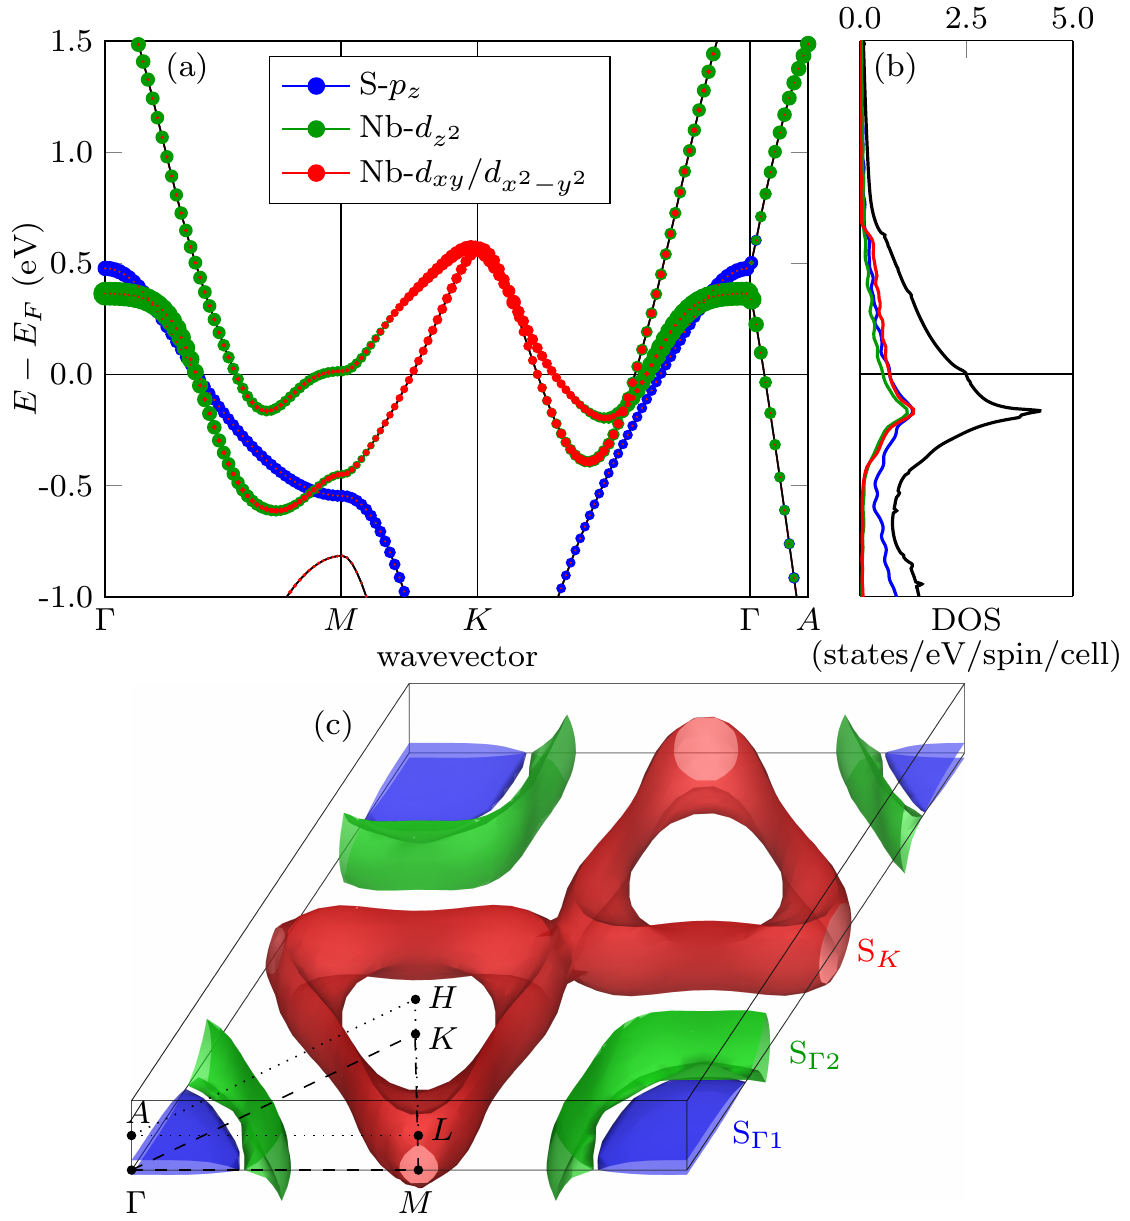
\includegraphics[width=\columnwidth]{fig1}
  \caption{(Color online) 
  (a) Calculated band structure of $2H$-NbS$_2$, with the orbital contributions proportional to the size of the colored dots, as indicated in the legend: S-$p_z$ (blue), Nb-$d_{z^2}$ (green) and Nb-$d_{xy}/d_{x^2-y^2}$ (red). 
  (b) Corresponding DOS and decomposition into atomic orbitals, using the same color code as in (a). The black line is the total DOS. 
  (c) Fermi surface showing the three distinct Fermi surface sheets labeled as S$_{\Gamma_1}$ (blue), S$_{\Gamma_2}$ (green), and S$_K$ (red); as well as the high-symmetry points in the Brillouin zone.}
  \label{fig1}
  \end{figure}

Figures~\ref{fig2}(a) and (b) show the calculated phonon dispersion relations of 2$H$-NbS$_2$. In the harmonic approximation the two lowest-energy vibrational modes near the $M$ and $L$ points of the Brillouin zone have imaginary frequencies, as shown in Supplemental Fig.~S2(f)-(g)~\cite{Note3}. For each of these modes we performed fully anharmonic calculations by mapping the DFT potential energy surface, and used the renormalized anharmonic frequencies in all calculations of phonon dispersions and EPIs. The resulting dispersion relations are in good agreement with inelastic X-ray scattering
experiments~\cite{leroux_anharmonic_2012}. At the $M$ point the anharmonic modes have A$_g$ and B$_u$ symmetry, respectively. The DFT potential energy surfaces of these modes correspond to symmetric double-wells, and can be identified with the modes which drive the CDW instability in related TMDs~\cite{moncton_neutron_1977,calandra_effect_2009,weber_extended_2011,leroux_strong_2015}. Details about these calculations and comparisons with other methods~\cite{born_fest._1951,hooton_li._1955,koehler_theory_1966,lam_ab_1982,souvatzis_entropy_2008,errea_first-principles_2013,giustino_materials_2014} are provided in the Supplemental Material~\cite{Note3}.

  \begin{figure}
  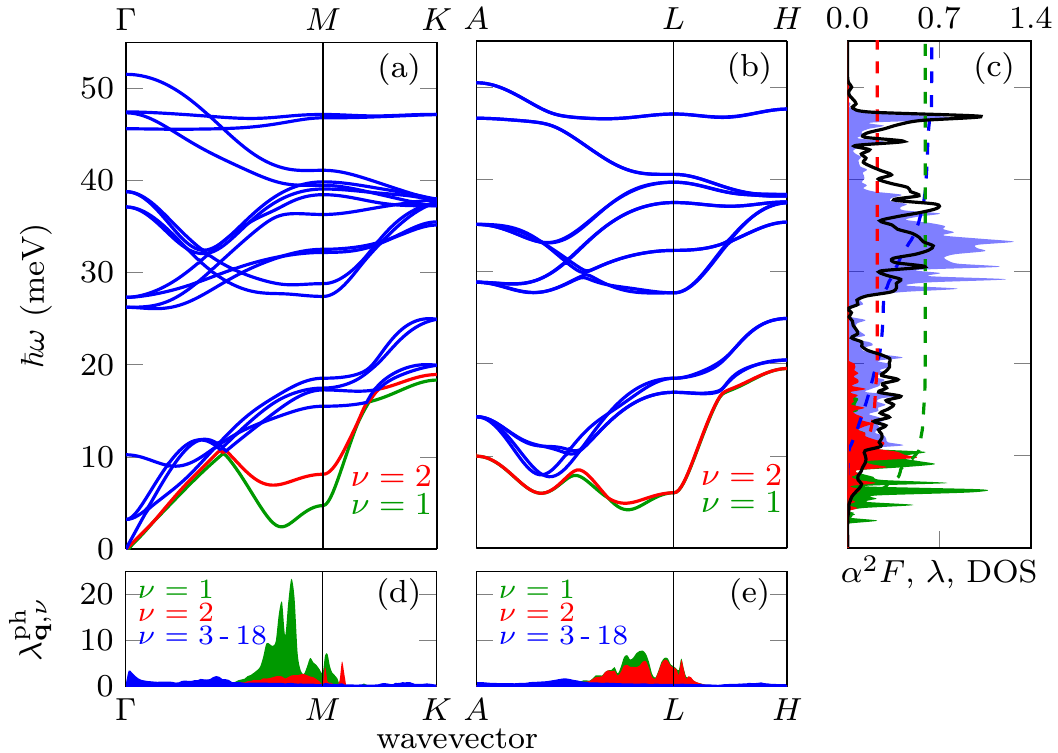
\includegraphics[width=\columnwidth]{fig2}
  \caption{(Color online) 
  (a)-(b) Calculated phonon dispersion relations of $2H$-NbS$_2$ for the first mode ($\nu=1$, green), the second mode ($\nu=2$, red), and modes $\nu=3-18$ (blue).
  (c) Calculated vibrational DOS (solid, black line), isotropic Eliashberg function $\alpha^2 F(\omega)$ (shaded areas) and 
  cumulative EPI strength $\lambda(\omega)$ (dashed lines). The blue curves are for modes $3-18$, and the green and red curves are for the two lowest-energy phonons.
  (d)-(e) The mode-resolved EPI strength $\lambda^{\rm ph}_{\mathbf{q},\nu}$ for the phonon modes in (a)-(b).
  }
  \label{fig2}
  \end{figure}

%
In Fig.~\ref{fig2}(d)-(e) we show the wavevector- and mode-resolved electron-phonon coupling strength $\lambda^{\rm ph}_{\mathbf{q},\nu}$ along high-symmetry lines.
%
We see that the two anharmonic branches exhibit anomalously large EPIs (up to \mbox{$\lambda^{\rm ph}_{\mathbf{q},\nu=1} =23.5$}). In order to check the weight of these modes on the total EPI, we show in Fig.~\ref{fig2}(c) the isotropic Eliashberg function $\alpha^2F(\omega)$~\cite{ponce_epw:_2016} separated into contributions arising from the two low-energy anharmonic modes (green and red); and the remaining modes (blue). The corresponding 
breakdown of the total EPI strength [$\lambda = 2\int_{0}^{\infty} \alpha^2 F(\omega)/\omega \; d\omega$] is shown by the dashed lines; this analysis indicates that the anharmonic modes contribute more than 50\% to the total interaction strength. At variance with these modes, the contributions of all other modes are relatively homogeneous and follow the vibrational DOS [Fig.~\ref{fig2}(c)].

  \begin{figure}
  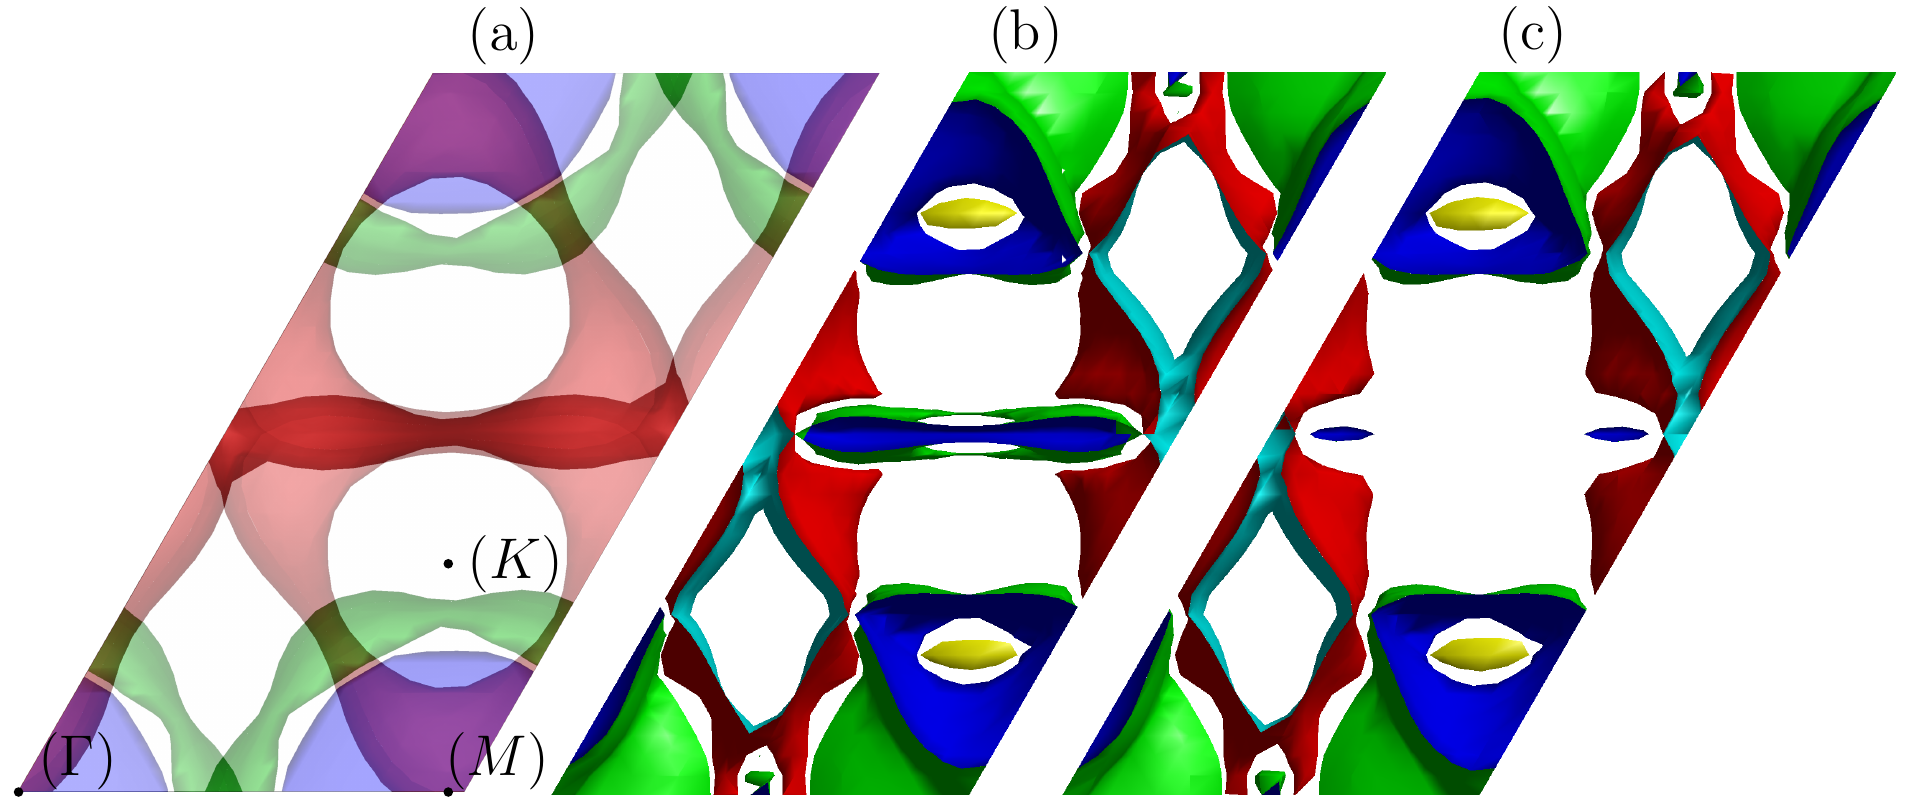
\includegraphics[width=\columnwidth]{fig3}
  \caption{
  (Color online)
  (a) Sketch of the folded FS of the 2$\times$1$\times$1 supercell, obtained by overlaying two FSs of the crystal unit cell. The high-symmetry points are indicated in brackets since they refer to the crystal Brillouin zone.
  (b) Calculated FS of the 2$\times$1$\times$1 supercell in the ground-state structure.
  (c) Calculated FS of the 2$\times$1$\times$1 supercell after displacing the atoms according to the B$_u$ phonon mode at $M$, so as to place the structure in one of the minima of the double-well potential.
  }
  \label{fig3}
  \end{figure}

Anomalous EPI strengths of selected phonons can arise either from Fermi surface nesting effects~\cite{kohn_image_1959}, or from the breaking of electronic degeneracies by lattice fluctuations and the consequent removal of electronic weight from the DOS close to the Fermi level~\cite{katsnelson_singularities_1994}, in analogy to the dynamical Jahn-Teller effect in molecules~\cite{bersuker_jahn-teller_2006}.
To determine which mechanism is active in the case of $2H$-NbS$_2$, we calculated
the Fermi surface nesting function~\cite{ponce_epw:_2016,heil_accurate_2014}. By inspecting this function
in Supplemental Fig.~S3~\cite{Note3} we see that there are no obvious nesting vectors in this system, likely because the sides of the triangular Fermi pocket S$_K$ are bulging inwards (Fig.~\ref{fig1}). 
%
Therefore we rule out nesting as a possible cause of strong EPIs in the anharmonic modes. This is in line with previous reports on other TMDs~\cite{johannes_fs_2006, valla_quasiparticle_2004, weber_extended_2011, calandra_charge-density_2011}. 
%
In order to test the second mechanism, we focused on the B$_u$ mode at the $M$ point. We doubled the NbS$_2$ unit cell along the $\Gamma M$ direction so as to fold $M$ into $\Gamma$, and calculated band structures, DOS and Fermi surfaces with or without a frozen B$_u$ phonon~\footnote{Calculations with frozen A$_g$ phonon lead to similar results, as shown in Supplemental Fig.~S4~\cite{Note3}}. This phonon induces avoided crossings near the Fermi level in regions which correspond to the centers of the triangular Fermi arcs S$_K$ in Fig.~\ref{fig1}(c).
%
The deformation of the band structure is accompanied by a suppression of large parts of the Fermi surface in the supercell [as shown in Fig.~\ref{fig3} and Supplemental Fig.~S4~\cite{Note3}] and leads to the removal of the pronounced shoulder in the DOS close to the Fermi energy of the undistorted structure [see Fig.~\ref{fig1} and Supplemental Fig.~S5~\cite{Note3}]. As pointed out in Refs.~\onlinecite{katsnelson_singularities_1994,katsnelson_anomalies_1985}, such changes in the electronic structure are indicative of a phonon softening and a latent lattice instability, and is in line with our findings of Fermi-surface EPI hot spots precisely in the middle of the triangular sides of S$_K$.

We now move to the superconducting properties of 2$H$-NbS$_2$. Figure~\ref{fig4}(a) shows the distribution of temperature-dependent superconducting gaps on the Fermi surface, as calculated using the anisotropic \textit{ab initio} Migdal-Eliashberg theory. Our calculations using the DFT band structure 
yield a critical temperature \mbox{$T_{\rm c} = 18.6$~K} and a maximum zero-temperature superconducting gap \mbox{$\Delta = 4.2$~meV}, overestimating the experimental values of 5.7~K and 0.97~meV, respectively~\cite{guillamon_superconducting_2008}. The origin of this discrepancy
will be discussed further down; for now, in order to facilitate comparison with experiment,
we apply the empirical scaling factors $5.7/18.6$ and $0.97/4.2$, respectively.

  \begin{figure}
  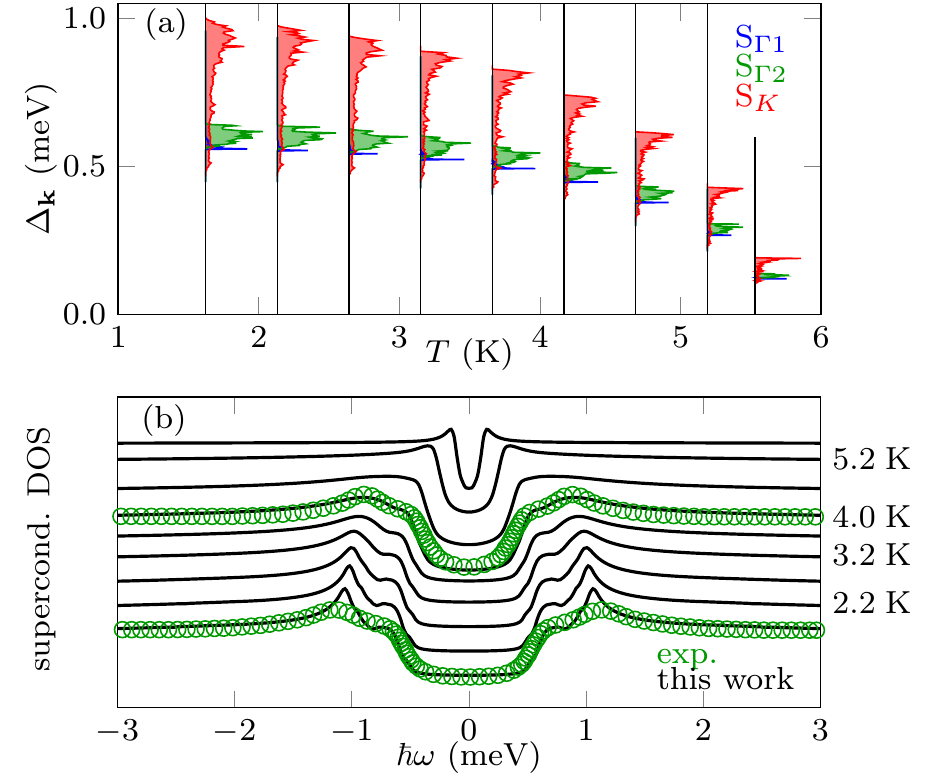
\includegraphics[width=\columnwidth]{fig4}
  \caption{(Color online) 
  (a) Energy distribution of the superconducting gap $\Delta_{\bf k}$ of $2H$-NbS$_2$ as a function of temperature, calculated within the anisotropic {\it ab initio} Migdal-Eliashberg theory including Coulomb interactions. The colors indicate data belonging to different Fermi surface sheets.
  (b) Calculated DOS in the superconducting phase of $2H$-NbS$_2$ (black lines), compared with tunneling data from Ref.~\onlinecite{guillamon_superconducting_2008} (green circles), for $T=1.8$~K and $T=4.0$~K. In both panels, to facilitate comparison with experiment, {\it the theoretical temperature and gaps were scaled by the factors $5.7/18.6$ and $0.97/4.2$, respectively}.}
  \label{fig4}
  \end{figure}

The superconducting gaps in Fig.~\ref{fig4}(a) are seen to follow the standard BCS-type temperature dependence. At each temperature the gaps cluster around two distinct values, indicating that 2$H$-NbS$_2$ is a two-gap superconductor. The smaller gap is associated with the Fermi sheets S$_{\Gamma_1}$ and S$_{\Gamma_2}$, while the larger gap belongs to S$_{K}$. From the gaps we calculate the superconducting DOS, and in Fig.~\ref{fig4}(b) we compare our results to the tunneling experiments of Ref.~\onlinecite{guillamon_superconducting_2008}. The agreement between our calculations and experiments is very good (apart from the empirical scaling discussed above), and confirms that the peak around 1.0~meV and the shoulder around 0.6~meV in the tunneling data taken at 1.8~K are to be associated with two distinct superconducting gaps on the $\Gamma$-centered and on the $K$-centered Fermi surface pockets.
Our finding of two distinct superconducting gaps is also in line with the anomalous temperature dependence of the specific heat~\cite{kacmarcik_specific_2010} and the pressure dependence of the upper critical field~\cite{tissen_pressure_2013}. 

  \begin{figure}
  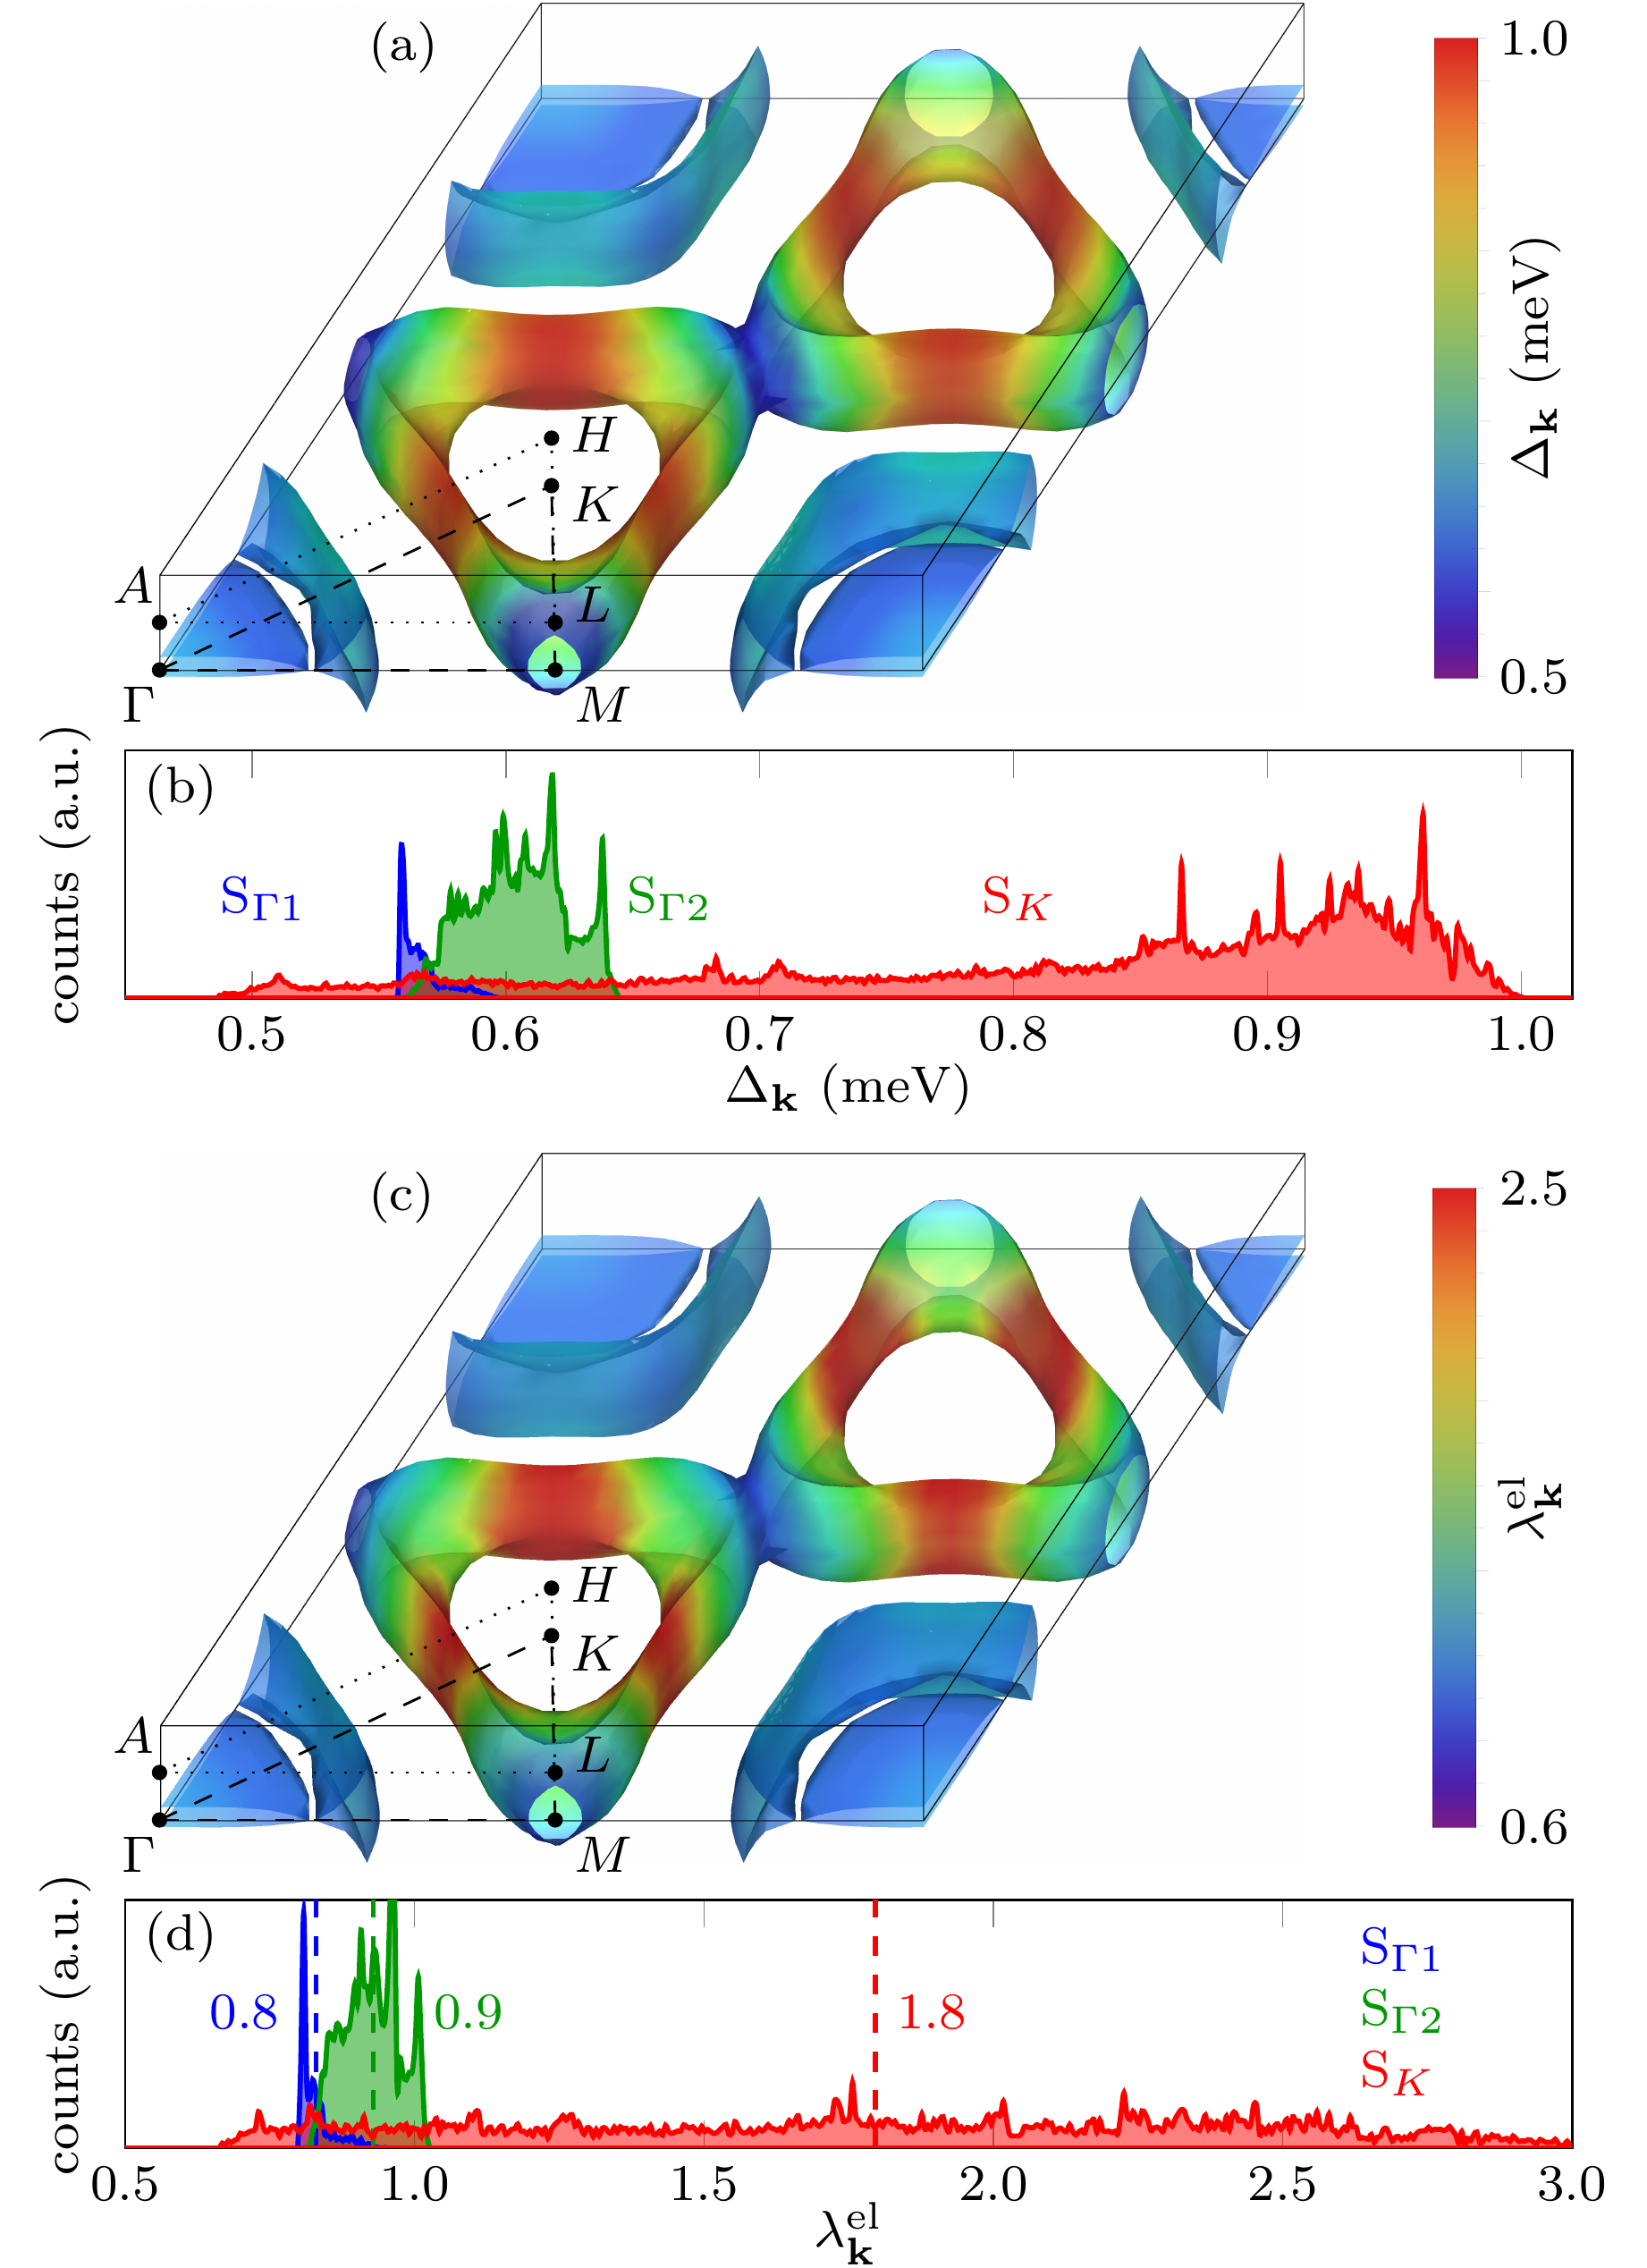
\includegraphics[width=\columnwidth]{fig5.png}
  \caption{(Color online)
  (a) Momentum-resolved superconducting gap $\Delta_{\bf k}$ on the Fermi surface of
  $2H$-NbS$_2$, calculated within the {\it ab initio} Migdal-Eliashberg theory for $T=1.7$~K.
  (b) Energy distribution of the superconducting gap $\Delta_{\bf k}$, color-coded by 
  Fermi surface sheet: S$_{\Gamma_1}$ (blue), S$_{\Gamma_2}$ (green), and S$_{K}$ (red). The values for the gaps were scaled as in Fig.~\ref{fig4}.
  (c)  Momentum-resolved EPI strength $\lambda^{\rm el}_{\bf k}$ on the Fermi surface of
  $2H$-NbS$_2$. 
  (d) Distribution of the EPI strength $\lambda^{\rm el}_{\bf k}$ by magnitude, color-coded by Fermi surface sheet as in (b).
  }
  \label{fig5}
  \end{figure}

Figure~\ref{fig5}(a) shows the momentum-resolved superconducting gap on the Fermi surface. We observe finite values for $\Delta_\mathbf{k}$ on the whole FS, therefore the FS is fully gapped below the critical temperature. The gaps on the S$_{\Gamma_1}$ and S$_{\Gamma_2}$ sheets exhibit narrow distributions centered around 0.57~meV and 0.56-0.65~meV, respectively. In contrast, the gap on the S$_{K}$ sheet is highly anisotropic and varies over the wide range 0.5-1.0~meV [Fig.~\ref{fig5}(b)]. By recalling the orbital analysis of the Fermi surface in Fig.~\ref{fig1} we conclude that low values of the superconducting gaps are found on those regions of the Fermi surface with out-of-plane orbital character (S-$p_z$ and Nb-$d_{z^2}$), while large values
correspond to regions with in-plane character (\mbox{Nb-$d_{xy}$} and $d_{x^2-y^2}$).

The regions of the Fermi surface with the largest superconducting gap coincide with
the hot spots of the electronic EPI parameter $\lambda^{\rm el}_{\bf k}$, as shown in Fig.~\ref{fig5}(c). In particular the EPI strength on the $\Gamma$-centered pockets exhibits a narrow distribution around $\lambda^{\rm el}_{\bf k}=0.8$-0.9, while that on the $K$-centered pocket covers the wide range from $\lambda^{\rm el}_{\bf k}=0.6$ to $\lambda^{\rm el}_{\bf k}=3.0$. The resulting average EPI parameter is $\lambda^{\rm el} = 1.46$. 
We emphasize that, while $\lambda^{\rm ph}_{\bf k,\nu}$ (Fig.~\ref{fig2}) and $\lambda^{\rm el}_{\bf k}$ (Fig.~\ref{fig5}) are related, they are not the same quantity. A detailed discussion of these quantities can be found in Ref.~\onlinecite{giustino_electron-phonon_2016}.
%
From this analysis it is clear that the two anharmonic modes contribute significantly to creating electron-phonon hot spots on the triangular arcs of the Fermi surface. While no charge ordering has been observed in $2H$-NbS$_2$ thus far, our findings clearly indicate that the EPI with the anharmonic phonons places this system very close to a lattice instability~\cite{overhauser_observability_1971}. This conclusion is further supported by the Fermi surface contribution to the adiabatic phonon self-energy~\cite{zhang_nonlocal_2005} presented in Supplemental Fig.~S6~\cite{Note3}. Based on these considerations we propose that superconductivity in $2H$-NbS$_2$ is driven by the same EPI that underlies a `latent' CDW instability, i.e. a CDW that is possibly quenched by quantum fluctuations.

We now come back to the overestimation of the measured critical temperature in our calculations. 
%
At present it is unclear whether this overestimation relates to an inadequate description of anharmonic effects, to the use of the Migdal approximation, to the approximate treatment of retardation effects, or to the assumption of constant DOS near the Fermi level in the Eliashberg theory~\cite{margine_anisotropic_2013}.
In order to test the sensitivity of our results to some of these effects, we repeated
our calculations (i) by varying the frequency of the anharmonic modes, and (ii) by
varying the DOS via a rigid shift of the Fermi level. Supplemental Fig.~S7~\cite{Note3} shows that our calculated $T_{\rm c}$ is insensitive to the frequency of the anharmonic modes over a wide range, therefore we can exclude this scenario. In contrast, Supplemental Fig.~S8~\cite{Note3} shows that the critical temperature is in better agreement with experiments if we raise the Fermi level by only 200~meV. 
Motivated by this observation we performed quasiparticle GW calculations of the band structure of NbS$_2$~\cite{giustino_gw_2010,lambert_ab_2013,giustino_electron-phonon_2016,hybertsen_electron_1986,godby_metal-insulator_1989,onida_electronic_2002}. Supplemental Fig.~S9~\cite{Note3} shows that GW quasiparticle corrections reduce the DOS at the Fermi energy by 18\% with respect to our DFT calculations. By repeating our Eliashberg calculations with the corrected $N_{\rm F}$ and $\mu^*$ we find that the critical temperature also decreases by 
18\%. For completeness the superconducting gap calculated after including quasiparticle corrections is shown in
Supplemental Fig.~S10~\cite{Note3}.
Our most accurate value, $T_{\rm c} = 15.3$\;K, is in better agreement with experiment.

In conclusion, we used the anisotropic {\it ab initio} Migdal-Eliashberg theory including
Coulomb interactions to elucidate the nature of the superconducting pairing in 2$H$-NbS$_2$. 
Our calculations indicate that a large contribution to the pairing comes from EPI hot spots on the triangular Fermi surface arcs, which signal a latent CDW instability. 
We successfully explained tunneling measurements in terms of two superconducting gaps, a large one associated with in-plane Nb orbitals, and a small one related to the out-of-plane orbitals of Nb and S. 
More generally, our work highlights the importance of determining accurate low-energy band structures
and Fermi surfaces beyond DFT in order to achieve a fully {\it ab initio} description of the
pairing mechanism in TMDs.




\begin{acknowledgments}
We gratefully acknowledge fruitful discussions with M. A. Perez Osorio, M. Zacharias, N. Zibouche, C. Verdi and L. Boeri.
This work was supported by the Austrian Science Fund (FWF) Project No. J 3806-N36, 
the Leverhulme Trust (Grant RL-2012-001), the UK Engineering and Physical Sciences Research 
Council (grants No. EP/J009857/1 and EP/M020517/1), the European Union's Horizon 2020 
programme under grant No.~696656 GrapheneCore1, the University of Oxford Advanced Research Computing (ARC) facility (http://dx.doi.org/810.5281/zenodo.22558) and the ARCHER UK National Supercomputing Service under the `AMSEC' Leadership project.
\end{acknowledgments}


\bibliographystyle{apsrev4-1}
% \bibliography{library}
%merlin.mbs apsrev4-1.bst 2010-07-25 4.21a (PWD, AO, DPC) hacked
%Control: key (0)
%Control: author (72) initials jnrlst
%Control: editor formatted (1) identically to author
%Control: production of article title (-1) disabled
%Control: page (0) single
%Control: year (1) truncated
%Control: production of eprint (0) enabled
\begin{thebibliography}{60}%
\makeatletter
\providecommand \@ifxundefined [1]{%
 \@ifx{#1\undefined}
}%
\providecommand \@ifnum [1]{%
 \ifnum #1\expandafter \@firstoftwo
 \else \expandafter \@secondoftwo
 \fi
}%
\providecommand \@ifx [1]{%
 \ifx #1\expandafter \@firstoftwo
 \else \expandafter \@secondoftwo
 \fi
}%
\providecommand \natexlab [1]{#1}%
\providecommand \enquote  [1]{``#1''}%
\providecommand \bibnamefont  [1]{#1}%
\providecommand \bibfnamefont [1]{#1}%
\providecommand \citenamefont [1]{#1}%
\providecommand \href@noop [0]{\@secondoftwo}%
\providecommand \href [0]{\begingroup \@sanitize@url \@href}%
\providecommand \@href[1]{\@@startlink{#1}\@@href}%
\providecommand \@@href[1]{\endgroup#1\@@endlink}%
\providecommand \@sanitize@url [0]{\catcode `\\12\catcode `\$12\catcode
  `\&12\catcode `\#12\catcode `\^12\catcode `\_12\catcode `\%12\relax}%
\providecommand \@@startlink[1]{}%
\providecommand \@@endlink[0]{}%
\providecommand \url  [0]{\begingroup\@sanitize@url \@url }%
\providecommand \@url [1]{\endgroup\@href {#1}{\urlprefix }}%
\providecommand \urlprefix  [0]{URL }%
\providecommand \Eprint [0]{\href }%
\providecommand \doibase [0]{http://dx.doi.org/}%
\providecommand \selectlanguage [0]{\@gobble}%
\providecommand \bibinfo  [0]{\@secondoftwo}%
\providecommand \bibfield  [0]{\@secondoftwo}%
\providecommand \translation [1]{[#1]}%
\providecommand \BibitemOpen [0]{}%
\providecommand \bibitemStop [0]{}%
\providecommand \bibitemNoStop [0]{.\EOS\space}%
\providecommand \EOS [0]{\spacefactor3000\relax}%
\providecommand \BibitemShut  [1]{\csname bibitem#1\endcsname}%
\let\auto@bib@innerbib\@empty
%</preamble>
\bibitem [{\citenamefont {Sipos}\ \emph {et~al.}(2008)\citenamefont {Sipos},
  \citenamefont {Kusmartseva}, \citenamefont {Akrap}, \citenamefont {Berger},
  \citenamefont {For\'{o}},\ and\ \citenamefont {Tuti\v{s}}}]{sipos_mott_2008}%
  \BibitemOpen
  \bibfield  {author} {\bibinfo {author} {\bibfnamefont {B.}~\bibnamefont
  {Sipos}}, \bibinfo {author} {\bibfnamefont {A.~F.}\ \bibnamefont
  {Kusmartseva}}, \bibinfo {author} {\bibfnamefont {A.}~\bibnamefont {Akrap}},
  \bibinfo {author} {\bibfnamefont {H.}~\bibnamefont {Berger}}, \bibinfo
  {author} {\bibfnamefont {L.}~\bibnamefont {For\'{o}}}, \ and\ \bibinfo
  {author} {\bibfnamefont {E.}~\bibnamefont {Tuti\v{s}}},\ }\href {\doibase
  10.1038/nmat2318} {\bibfield  {journal} {\bibinfo  {journal} {Nat. Mater.}\
  }\textbf {\bibinfo {volume} {7}},\ \bibinfo {pages} {960} (\bibinfo {year}
  {2008})}\BibitemShut {NoStop}%
\bibitem [{\citenamefont {Wang}\ \emph {et~al.}(2012)\citenamefont {Wang},
  \citenamefont {Kalantar-Zadeh}, \citenamefont {Kis}, \citenamefont
  {Coleman},\ and\ \citenamefont {Strano}}]{wang_electronics_2012}%
  \BibitemOpen
  \bibfield  {author} {\bibinfo {author} {\bibfnamefont {Q.~H.}\ \bibnamefont
  {Wang}}, \bibinfo {author} {\bibfnamefont {K.}~\bibnamefont
  {Kalantar-Zadeh}}, \bibinfo {author} {\bibfnamefont {A.}~\bibnamefont {Kis}},
  \bibinfo {author} {\bibfnamefont {J.~N.}\ \bibnamefont {Coleman}}, \ and\
  \bibinfo {author} {\bibfnamefont {M.~S.}\ \bibnamefont {Strano}},\ }\href
  {\doibase 10.1038/nnano.2012.193} {\bibfield  {journal} {\bibinfo  {journal}
  {Nat. Nanotechnol.}\ }\textbf {\bibinfo {volume} {7}},\ \bibinfo {pages}
  {699} (\bibinfo {year} {2012})}\BibitemShut {NoStop}%
\bibitem [{\citenamefont {Geim}\ and\ \citenamefont
  {Grigorieva}(2013)}]{geim_van_2013}%
  \BibitemOpen
  \bibfield  {author} {\bibinfo {author} {\bibfnamefont {A.~K.}\ \bibnamefont
  {Geim}}\ and\ \bibinfo {author} {\bibfnamefont {I.~V.}\ \bibnamefont
  {Grigorieva}},\ }\href {\doibase 10.1038/nature12385} {\bibfield  {journal}
  {\bibinfo  {journal} {Nature}\ }\textbf {\bibinfo {volume} {499}},\ \bibinfo
  {pages} {419} (\bibinfo {year} {2013})}\BibitemShut {NoStop}%
\bibitem [{\citenamefont {Klemm}(2015)}]{klemm_pristine_2015}%
  \BibitemOpen
  \bibfield  {author} {\bibinfo {author} {\bibfnamefont {R.~A.}\ \bibnamefont
  {Klemm}},\ }\href {\doibase 10.1016/j.physc.2015.02.023} {\bibfield
  {journal} {\bibinfo  {journal} {Physica C}\ }\textbf {\bibinfo {volume}
  {514}},\ \bibinfo {pages} {86} (\bibinfo {year} {2015})}\BibitemShut
  {NoStop}%
\bibitem [{\citenamefont {Wilson}\ and\ \citenamefont
  {Yoffe}(1969)}]{wilson_transition_1969}%
  \BibitemOpen
  \bibfield  {author} {\bibinfo {author} {\bibfnamefont {J.}~\bibnamefont
  {Wilson}}\ and\ \bibinfo {author} {\bibfnamefont {A.}~\bibnamefont {Yoffe}},\
  }\href {\doibase 10.1080/00018736900101307} {\bibfield  {journal} {\bibinfo
  {journal} {Adv. Phys.}\ }\textbf {\bibinfo {volume} {18}},\ \bibinfo {pages}
  {193} (\bibinfo {year} {1969})}\BibitemShut {NoStop}%
\bibitem [{\citenamefont {Moncton}\ \emph {et~al.}(1975)\citenamefont
  {Moncton}, \citenamefont {Axe},\ and\ \citenamefont
  {DiSalvo}}]{moncton_study_1975}%
  \BibitemOpen
  \bibfield  {author} {\bibinfo {author} {\bibfnamefont {D.~E.}\ \bibnamefont
  {Moncton}}, \bibinfo {author} {\bibfnamefont {J.~D.}\ \bibnamefont {Axe}}, \
  and\ \bibinfo {author} {\bibfnamefont {F.~J.}\ \bibnamefont {DiSalvo}},\
  }\href {\doibase 10.1103/PhysRevLett.34.734} {\bibfield  {journal} {\bibinfo
  {journal} {Phys. Rev. Lett.}\ }\textbf {\bibinfo {volume} {34}},\ \bibinfo
  {pages} {734} (\bibinfo {year} {1975})}\BibitemShut {NoStop}%
\bibitem [{\citenamefont {Valla}\ \emph {et~al.}(2004)\citenamefont {Valla},
  \citenamefont {Fedorov}, \citenamefont {Johnson}, \citenamefont {Glans},
  \citenamefont {McGuinness}, \citenamefont {Smith}, \citenamefont {Andrei},\
  and\ \citenamefont {Berger}}]{valla_quasiparticle_2004}%
  \BibitemOpen
  \bibfield  {author} {\bibinfo {author} {\bibfnamefont {T.}~\bibnamefont
  {Valla}}, \bibinfo {author} {\bibfnamefont {A.~V.}\ \bibnamefont {Fedorov}},
  \bibinfo {author} {\bibfnamefont {P.~D.}\ \bibnamefont {Johnson}}, \bibinfo
  {author} {\bibfnamefont {P.-A.}\ \bibnamefont {Glans}}, \bibinfo {author}
  {\bibfnamefont {C.}~\bibnamefont {McGuinness}}, \bibinfo {author}
  {\bibfnamefont {K.~E.}\ \bibnamefont {Smith}}, \bibinfo {author}
  {\bibfnamefont {E.~Y.}\ \bibnamefont {Andrei}}, \ and\ \bibinfo {author}
  {\bibfnamefont {H.}~\bibnamefont {Berger}},\ }\href {\doibase
  10.1103/PhysRevLett.92.086401} {\bibfield  {journal} {\bibinfo  {journal}
  {Phys. Rev. Lett.}\ }\textbf {\bibinfo {volume} {92}},\ \bibinfo {pages}
  {086401} (\bibinfo {year} {2004})}\BibitemShut {NoStop}%
\bibitem [{\citenamefont {Weber}\ \emph {et~al.}(2011)\citenamefont {Weber},
  \citenamefont {Rosenkranz}, \citenamefont {Castellan}, \citenamefont
  {Osborn}, \citenamefont {Hott}, \citenamefont {Heid}, \citenamefont {Bohnen},
  \citenamefont {Egami}, \citenamefont {Said},\ and\ \citenamefont
  {Reznik}}]{weber_extended_2011}%
  \BibitemOpen
  \bibfield  {author} {\bibinfo {author} {\bibfnamefont {F.}~\bibnamefont
  {Weber}}, \bibinfo {author} {\bibfnamefont {S.}~\bibnamefont {Rosenkranz}},
  \bibinfo {author} {\bibfnamefont {J.-P.}\ \bibnamefont {Castellan}}, \bibinfo
  {author} {\bibfnamefont {R.}~\bibnamefont {Osborn}}, \bibinfo {author}
  {\bibfnamefont {R.}~\bibnamefont {Hott}}, \bibinfo {author} {\bibfnamefont
  {R.}~\bibnamefont {Heid}}, \bibinfo {author} {\bibfnamefont {K.-P.}\
  \bibnamefont {Bohnen}}, \bibinfo {author} {\bibfnamefont {T.}~\bibnamefont
  {Egami}}, \bibinfo {author} {\bibfnamefont {A.~H.}\ \bibnamefont {Said}}, \
  and\ \bibinfo {author} {\bibfnamefont {D.}~\bibnamefont {Reznik}},\ }\href
  {\doibase 10.1103/PhysRevLett.107.107403} {\bibfield  {journal} {\bibinfo
  {journal} {Phys. Rev. Lett.}\ }\textbf {\bibinfo {volume} {107}},\ \bibinfo
  {pages} {107403} (\bibinfo {year} {2011})}\BibitemShut {NoStop}%
\bibitem [{\citenamefont {Calandra}\ and\ \citenamefont
  {Mauri}(2011)}]{calandra_charge-density_2011}%
  \BibitemOpen
  \bibfield  {author} {\bibinfo {author} {\bibfnamefont {M.}~\bibnamefont
  {Calandra}}\ and\ \bibinfo {author} {\bibfnamefont {F.}~\bibnamefont
  {Mauri}},\ }\href {\doibase 10.1103/PhysRevLett.106.196406} {\bibfield
  {journal} {\bibinfo  {journal} {Phys. Rev. Lett.}\ }\textbf {\bibinfo
  {volume} {106}},\ \bibinfo {pages} {196406} (\bibinfo {year}
  {2011})}\BibitemShut {NoStop}%
\bibitem [{\citenamefont {R\"{o}sner}\ \emph {et~al.}(2014)\citenamefont
  {R\"{o}sner}, \citenamefont {Haas},\ and\ \citenamefont
  {Wehling}}]{rosner_phase_2014}%
  \BibitemOpen
  \bibfield  {author} {\bibinfo {author} {\bibfnamefont {M.}~\bibnamefont
  {R\"{o}sner}}, \bibinfo {author} {\bibfnamefont {S.}~\bibnamefont {Haas}}, \
  and\ \bibinfo {author} {\bibfnamefont {T.~O.}\ \bibnamefont {Wehling}},\
  }\href {\doibase 10.1103/PhysRevB.90.245105} {\bibfield  {journal} {\bibinfo
  {journal} {Phys. Rev. B}\ }\textbf {\bibinfo {volume} {90}},\ \bibinfo
  {pages} {245105} (\bibinfo {year} {2014})}\BibitemShut {NoStop}%
\bibitem [{\citenamefont {Leroux}\ \emph {et~al.}(2015)\citenamefont {Leroux},
  \citenamefont {Errea}, \citenamefont {Le~Tacon}, \citenamefont {Souliou},
  \citenamefont {Garbarino}, \citenamefont {Cario}, \citenamefont {Bosak},
  \citenamefont {Mauri}, \citenamefont {Calandra},\ and\ \citenamefont
  {Rodi\`{e}re}}]{leroux_strong_2015}%
  \BibitemOpen
  \bibfield  {author} {\bibinfo {author} {\bibfnamefont {M.}~\bibnamefont
  {Leroux}}, \bibinfo {author} {\bibfnamefont {I.}~\bibnamefont {Errea}},
  \bibinfo {author} {\bibfnamefont {M.}~\bibnamefont {Le~Tacon}}, \bibinfo
  {author} {\bibfnamefont {S.-M.}\ \bibnamefont {Souliou}}, \bibinfo {author}
  {\bibfnamefont {G.}~\bibnamefont {Garbarino}}, \bibinfo {author}
  {\bibfnamefont {L.}~\bibnamefont {Cario}}, \bibinfo {author} {\bibfnamefont
  {A.}~\bibnamefont {Bosak}}, \bibinfo {author} {\bibfnamefont
  {F.}~\bibnamefont {Mauri}}, \bibinfo {author} {\bibfnamefont
  {M.}~\bibnamefont {Calandra}}, \ and\ \bibinfo {author} {\bibfnamefont
  {P.}~\bibnamefont {Rodi\`{e}re}},\ }\href {\doibase
  10.1103/PhysRevB.92.140303} {\bibfield  {journal} {\bibinfo  {journal} {Phys.
  Rev. B}\ }\textbf {\bibinfo {volume} {92}},\ \bibinfo {pages} {140303}
  (\bibinfo {year} {2015})}\BibitemShut {NoStop}%
\bibitem [{\citenamefont {Das}\ and\ \citenamefont
  {Dolui}(2015)}]{das_superconducting_2015}%
  \BibitemOpen
  \bibfield  {author} {\bibinfo {author} {\bibfnamefont {T.}~\bibnamefont
  {Das}}\ and\ \bibinfo {author} {\bibfnamefont {K.}~\bibnamefont {Dolui}},\
  }\href {\doibase 10.1103/PhysRevB.91.094510} {\bibfield  {journal} {\bibinfo
  {journal} {Phys. Rev. B}\ }\textbf {\bibinfo {volume} {91}},\ \bibinfo
  {pages} {094510} (\bibinfo {year} {2015})}\BibitemShut {NoStop}%
\bibitem [{\citenamefont {Naito}\ and\ \citenamefont
  {Tanaka}(1982)}]{naito_electrical_1982}%
  \BibitemOpen
  \bibfield  {author} {\bibinfo {author} {\bibfnamefont {M.}~\bibnamefont
  {Naito}}\ and\ \bibinfo {author} {\bibfnamefont {S.}~\bibnamefont {Tanaka}},\
  }\href {\doibase 10.1143/JPSJ.51.219} {\bibfield  {journal} {\bibinfo
  {journal} {J. Phys. Soc. Jpn.}\ }\textbf {\bibinfo {volume} {51}},\ \bibinfo
  {pages} {219} (\bibinfo {year} {1982})}\BibitemShut {NoStop}%
\bibitem [{\citenamefont {Guillam\'{o}n}\ \emph {et~al.}(2008)\citenamefont
  {Guillam\'{o}n}, \citenamefont {Suderow}, \citenamefont {Vieira},
  \citenamefont {Cario}, \citenamefont {Diener},\ and\ \citenamefont
  {Rodi\`{e}re}}]{guillamon_superconducting_2008}%
  \BibitemOpen
  \bibfield  {author} {\bibinfo {author} {\bibfnamefont {I.}~\bibnamefont
  {Guillam\'{o}n}}, \bibinfo {author} {\bibfnamefont {H.}~\bibnamefont
  {Suderow}}, \bibinfo {author} {\bibfnamefont {S.}~\bibnamefont {Vieira}},
  \bibinfo {author} {\bibfnamefont {L.}~\bibnamefont {Cario}}, \bibinfo
  {author} {\bibfnamefont {P.}~\bibnamefont {Diener}}, \ and\ \bibinfo {author}
  {\bibfnamefont {P.}~\bibnamefont {Rodi\`{e}re}},\ }\href {\doibase
  10.1103/PhysRevLett.101.166407} {\bibfield  {journal} {\bibinfo  {journal}
  {Phys. Rev. Lett.}\ }\textbf {\bibinfo {volume} {101}},\ \bibinfo {pages}
  {166407} (\bibinfo {year} {2008})}\BibitemShut {NoStop}%
\bibitem [{\citenamefont {Liu}\ \emph {et~al.}(2014)\citenamefont {Liu},
  \citenamefont {Cai},\ and\ \citenamefont {Zhang}}]{liu_novel_2014}%
  \BibitemOpen
  \bibfield  {author} {\bibinfo {author} {\bibfnamefont {Z.-L.}\ \bibnamefont
  {Liu}}, \bibinfo {author} {\bibfnamefont {L.-C.}\ \bibnamefont {Cai}}, \ and\
  \bibinfo {author} {\bibfnamefont {X.-L.}\ \bibnamefont {Zhang}},\ }\href
  {\doibase 10.1016/j.jallcom.2014.05.013} {\bibfield  {journal} {\bibinfo
  {journal} {J. Alloys Compd.}\ }\textbf {\bibinfo {volume} {610}},\ \bibinfo
  {pages} {472} (\bibinfo {year} {2014})}\BibitemShut {NoStop}%
\bibitem [{\citenamefont {Nishio}\ \emph {et~al.}(1994)\citenamefont {Nishio},
  \citenamefont {Shirai}, \citenamefont {Suzuki},\ and\ \citenamefont
  {Motizuki}}]{nishio_role_1994}%
  \BibitemOpen
  \bibfield  {author} {\bibinfo {author} {\bibfnamefont {Y.}~\bibnamefont
  {Nishio}}, \bibinfo {author} {\bibfnamefont {M.}~\bibnamefont {Shirai}},
  \bibinfo {author} {\bibfnamefont {N.}~\bibnamefont {Suzuki}}, \ and\ \bibinfo
  {author} {\bibfnamefont {K.}~\bibnamefont {Motizuki}},\ }\href {\doibase
  10.1143/JPSJ.63.156} {\bibfield  {journal} {\bibinfo  {journal} {J. Phys.
  Soc. Jpn.}\ }\textbf {\bibinfo {volume} {63}},\ \bibinfo {pages} {156}
  (\bibinfo {year} {1994})}\BibitemShut {NoStop}%
\bibitem [{\citenamefont {Moncton}\ \emph {et~al.}(1977)\citenamefont
  {Moncton}, \citenamefont {Axe},\ and\ \citenamefont
  {DiSalvo}}]{moncton_neutron_1977}%
  \BibitemOpen
  \bibfield  {author} {\bibinfo {author} {\bibfnamefont {D.~E.}\ \bibnamefont
  {Moncton}}, \bibinfo {author} {\bibfnamefont {J.~D.}\ \bibnamefont {Axe}}, \
  and\ \bibinfo {author} {\bibfnamefont {F.~J.}\ \bibnamefont {DiSalvo}},\
  }\href {\doibase 10.1103/PhysRevB.16.801} {\bibfield  {journal} {\bibinfo
  {journal} {Phys. Rev. B}\ }\textbf {\bibinfo {volume} {16}},\ \bibinfo
  {pages} {801} (\bibinfo {year} {1977})}\BibitemShut {NoStop}%
\bibitem [{\citenamefont {Calandra}\ \emph {et~al.}(2009)\citenamefont
  {Calandra}, \citenamefont {Mazin},\ and\ \citenamefont
  {Mauri}}]{calandra_effect_2009}%
  \BibitemOpen
  \bibfield  {author} {\bibinfo {author} {\bibfnamefont {M.}~\bibnamefont
  {Calandra}}, \bibinfo {author} {\bibfnamefont {I.~I.}\ \bibnamefont {Mazin}},
  \ and\ \bibinfo {author} {\bibfnamefont {F.}~\bibnamefont {Mauri}},\ }\href
  {\doibase 10.1103/PhysRevB.80.241108} {\bibfield  {journal} {\bibinfo
  {journal} {Phys. Rev. B}\ }\textbf {\bibinfo {volume} {80}},\ \bibinfo
  {pages} {241108} (\bibinfo {year} {2009})}\BibitemShut {NoStop}%
\bibitem [{\citenamefont {Leroux}\ \emph {et~al.}(2012)\citenamefont {Leroux},
  \citenamefont {Le~Tacon}, \citenamefont {Calandra}, \citenamefont {Cario},
  \citenamefont {M\'{e}asson}, \citenamefont {Diener}, \citenamefont
  {Borrissenko}, \citenamefont {Bosak},\ and\ \citenamefont
  {Rodi\`{e}re}}]{leroux_anharmonic_2012}%
  \BibitemOpen
  \bibfield  {author} {\bibinfo {author} {\bibfnamefont {M.}~\bibnamefont
  {Leroux}}, \bibinfo {author} {\bibfnamefont {M.}~\bibnamefont {Le~Tacon}},
  \bibinfo {author} {\bibfnamefont {M.}~\bibnamefont {Calandra}}, \bibinfo
  {author} {\bibfnamefont {L.}~\bibnamefont {Cario}}, \bibinfo {author}
  {\bibfnamefont {M.-A.}\ \bibnamefont {M\'{e}asson}}, \bibinfo {author}
  {\bibfnamefont {P.}~\bibnamefont {Diener}}, \bibinfo {author} {\bibfnamefont
  {E.}~\bibnamefont {Borrissenko}}, \bibinfo {author} {\bibfnamefont
  {A.}~\bibnamefont {Bosak}}, \ and\ \bibinfo {author} {\bibfnamefont
  {P.}~\bibnamefont {Rodi\`{e}re}},\ }\href {\doibase
  10.1103/PhysRevB.86.155125} {\bibfield  {journal} {\bibinfo  {journal} {Phys.
  Rev. B}\ }\textbf {\bibinfo {volume} {86}},\ \bibinfo {pages} {155125}
  (\bibinfo {year} {2012})}\BibitemShut {NoStop}%
\bibitem [{\citenamefont {Perdew}\ and\ \citenamefont
  {Zunger}(1981)}]{perdew_self-interaction_1981}%
  \BibitemOpen
  \bibfield  {author} {\bibinfo {author} {\bibfnamefont {J.~P.}\ \bibnamefont
  {Perdew}}\ and\ \bibinfo {author} {\bibfnamefont {A.}~\bibnamefont
  {Zunger}},\ }\href {\doibase 10.1103/PhysRevB.23.5048} {\bibfield  {journal}
  {\bibinfo  {journal} {Phys. Rev. B}\ }\textbf {\bibinfo {volume} {23}},\
  \bibinfo {pages} {5048} (\bibinfo {year} {1981})}\BibitemShut {NoStop}%
\bibitem [{\citenamefont {Ceperley}\ and\ \citenamefont
  {Alder}(1980)}]{ceperley_ground_1980}%
  \BibitemOpen
  \bibfield  {author} {\bibinfo {author} {\bibfnamefont {D.~M.}\ \bibnamefont
  {Ceperley}}\ and\ \bibinfo {author} {\bibfnamefont {B.~J.}\ \bibnamefont
  {Alder}},\ }\href {\doibase 10.1103/PhysRevLett.45.566} {\bibfield  {journal}
  {\bibinfo  {journal} {Phys. Rev. Lett.}\ }\textbf {\bibinfo {volume} {45}},\
  \bibinfo {pages} {566} (\bibinfo {year} {1980})}\BibitemShut {NoStop}%
\bibitem [{\citenamefont {Giannozzi}\ \emph {et~al.}(2009)\citenamefont
  {Giannozzi}, \citenamefont {Baroni}, \citenamefont {Bonini}, \citenamefont
  {Calandra}, \citenamefont {Car}, \citenamefont {Cavazzoni}, \citenamefont
  {Ceresoli}, \citenamefont {Chiarotti}, \citenamefont {Cococcioni},
  \citenamefont {Dabo}, \citenamefont {Corso}, \citenamefont {Gironcoli},
  \citenamefont {Fabris}, \citenamefont {Fratesi}, \citenamefont {Gebauer},
  \citenamefont {Gerstmann}, \citenamefont {Gougoussis}, \citenamefont
  {Kokalj}, \citenamefont {Lazzeri}, \citenamefont {Martin-Samos},
  \citenamefont {Marzari}, \citenamefont {Mauri}, \citenamefont {Mazzarello},
  \citenamefont {Paolini}, \citenamefont {Pasquarello}, \citenamefont
  {Paulatto}, \citenamefont {Sbraccia}, \citenamefont {Scandolo}, \citenamefont
  {Sclauzero}, \citenamefont {Seitsonen}, \citenamefont {Smogunov},
  \citenamefont {Umari},\ and\ \citenamefont
  {Wentzcovitch}}]{giannozzi_quantum_2009}%
  \BibitemOpen
  \bibfield  {author} {\bibinfo {author} {\bibfnamefont {P.}~\bibnamefont
  {Giannozzi}}, \bibinfo {author} {\bibfnamefont {S.}~\bibnamefont {Baroni}},
  \bibinfo {author} {\bibfnamefont {N.}~\bibnamefont {Bonini}}, \bibinfo
  {author} {\bibfnamefont {M.}~\bibnamefont {Calandra}}, \bibinfo {author}
  {\bibfnamefont {R.}~\bibnamefont {Car}}, \bibinfo {author} {\bibfnamefont
  {C.}~\bibnamefont {Cavazzoni}}, \bibinfo {author} {\bibfnamefont
  {D.}~\bibnamefont {Ceresoli}}, \bibinfo {author} {\bibfnamefont {G.~L.}\
  \bibnamefont {Chiarotti}}, \bibinfo {author} {\bibfnamefont {M.}~\bibnamefont
  {Cococcioni}}, \bibinfo {author} {\bibfnamefont {I.}~\bibnamefont {Dabo}},
  \bibinfo {author} {\bibfnamefont {A.~D.}\ \bibnamefont {Corso}}, \bibinfo
  {author} {\bibfnamefont {S.~d.}\ \bibnamefont {Gironcoli}}, \bibinfo {author}
  {\bibfnamefont {S.}~\bibnamefont {Fabris}}, \bibinfo {author} {\bibfnamefont
  {G.}~\bibnamefont {Fratesi}}, \bibinfo {author} {\bibfnamefont
  {R.}~\bibnamefont {Gebauer}}, \bibinfo {author} {\bibfnamefont
  {U.}~\bibnamefont {Gerstmann}}, \bibinfo {author} {\bibfnamefont
  {C.}~\bibnamefont {Gougoussis}}, \bibinfo {author} {\bibfnamefont
  {A.}~\bibnamefont {Kokalj}}, \bibinfo {author} {\bibfnamefont
  {M.}~\bibnamefont {Lazzeri}}, \bibinfo {author} {\bibfnamefont
  {L.}~\bibnamefont {Martin-Samos}}, \bibinfo {author} {\bibfnamefont
  {N.}~\bibnamefont {Marzari}}, \bibinfo {author} {\bibfnamefont
  {F.}~\bibnamefont {Mauri}}, \bibinfo {author} {\bibfnamefont
  {R.}~\bibnamefont {Mazzarello}}, \bibinfo {author} {\bibfnamefont
  {S.}~\bibnamefont {Paolini}}, \bibinfo {author} {\bibfnamefont
  {A.}~\bibnamefont {Pasquarello}}, \bibinfo {author} {\bibfnamefont
  {L.}~\bibnamefont {Paulatto}}, \bibinfo {author} {\bibfnamefont
  {C.}~\bibnamefont {Sbraccia}}, \bibinfo {author} {\bibfnamefont
  {S.}~\bibnamefont {Scandolo}}, \bibinfo {author} {\bibfnamefont
  {G.}~\bibnamefont {Sclauzero}}, \bibinfo {author} {\bibfnamefont {A.~P.}\
  \bibnamefont {Seitsonen}}, \bibinfo {author} {\bibfnamefont {A.}~\bibnamefont
  {Smogunov}}, \bibinfo {author} {\bibfnamefont {P.}~\bibnamefont {Umari}}, \
  and\ \bibinfo {author} {\bibfnamefont {R.~M.}\ \bibnamefont {Wentzcovitch}},\
  }\href {\doibase 10.1088/0953-8984/21/39/395502} {\bibfield  {journal}
  {\bibinfo  {journal} {J. Phys. Condens. Matter}\ }\textbf {\bibinfo {volume}
  {21}},\ \bibinfo {pages} {395502} (\bibinfo {year} {2009})}\BibitemShut
  {NoStop}%
\bibitem [{\citenamefont {Giustino}\ \emph {et~al.}(2007)\citenamefont
  {Giustino}, \citenamefont {Cohen},\ and\ \citenamefont
  {Louie}}]{giustino_electron-phonon_2007}%
  \BibitemOpen
  \bibfield  {author} {\bibinfo {author} {\bibfnamefont {F.}~\bibnamefont
  {Giustino}}, \bibinfo {author} {\bibfnamefont {M.~L.}\ \bibnamefont {Cohen}},
  \ and\ \bibinfo {author} {\bibfnamefont {S.~G.}\ \bibnamefont {Louie}},\
  }\href {\doibase 10.1103/PhysRevB.76.165108} {\bibfield  {journal} {\bibinfo
  {journal} {Phys. Rev. B}\ }\textbf {\bibinfo {volume} {76}},\ \bibinfo
  {pages} {165108} (\bibinfo {year} {2007})}\BibitemShut {NoStop}%
\bibitem [{\citenamefont {Margine}\ and\ \citenamefont
  {Giustino}(2013)}]{margine_anisotropic_2013}%
  \BibitemOpen
  \bibfield  {author} {\bibinfo {author} {\bibfnamefont {E.~R.}\ \bibnamefont
  {Margine}}\ and\ \bibinfo {author} {\bibfnamefont {F.}~\bibnamefont
  {Giustino}},\ }\href {\doibase 10.1103/PhysRevB.87.024505} {\bibfield
  {journal} {\bibinfo  {journal} {Phys. Rev. B}\ }\textbf {\bibinfo {volume}
  {87}},\ \bibinfo {pages} {024505} (\bibinfo {year} {2013})}\BibitemShut
  {NoStop}%
\bibitem [{\citenamefont {Ponc\'{e}}\ \emph {et~al.}(2016)\citenamefont
  {Ponc\'{e}}, \citenamefont {Margine}, \citenamefont {Verdi},\ and\
  \citenamefont {Giustino}}]{ponce_epw:_2016}%
  \BibitemOpen
  \bibfield  {author} {\bibinfo {author} {\bibfnamefont {S.}~\bibnamefont
  {Ponc\'{e}}}, \bibinfo {author} {\bibfnamefont {E.~R.}\ \bibnamefont
  {Margine}}, \bibinfo {author} {\bibfnamefont {C.}~\bibnamefont {Verdi}}, \
  and\ \bibinfo {author} {\bibfnamefont {F.}~\bibnamefont {Giustino}},\ }\href
  {\doibase 10.1016/j.cpc.2016.07.028} {\bibfield  {journal} {\bibinfo
  {journal} {Comput. Phys. Commun.}\ }\textbf {\bibinfo {volume} {209}},\
  \bibinfo {pages} {116} (\bibinfo {year} {2016})}\BibitemShut {NoStop}%
\bibitem [{\citenamefont {Giustino}\ \emph {et~al.}(2010)\citenamefont
  {Giustino}, \citenamefont {Cohen},\ and\ \citenamefont
  {Louie}}]{giustino_gw_2010}%
  \BibitemOpen
  \bibfield  {author} {\bibinfo {author} {\bibfnamefont {F.}~\bibnamefont
  {Giustino}}, \bibinfo {author} {\bibfnamefont {M.~L.}\ \bibnamefont {Cohen}},
  \ and\ \bibinfo {author} {\bibfnamefont {S.~G.}\ \bibnamefont {Louie}},\
  }\href {\doibase 10.1103/PhysRevB.81.115105} {\bibfield  {journal} {\bibinfo
  {journal} {Phys. Rev. B}\ }\textbf {\bibinfo {volume} {81}},\ \bibinfo
  {pages} {115105} (\bibinfo {year} {2010})}\BibitemShut {NoStop}%
\bibitem [{\citenamefont {Lambert}\ and\ \citenamefont
  {Giustino}(2013)}]{lambert_ab_2013}%
  \BibitemOpen
  \bibfield  {author} {\bibinfo {author} {\bibfnamefont {H.}~\bibnamefont
  {Lambert}}\ and\ \bibinfo {author} {\bibfnamefont {F.}~\bibnamefont
  {Giustino}},\ }\href {\doibase 10.1103/PhysRevB.88.075117} {\bibfield
  {journal} {\bibinfo  {journal} {Phys. Rev. B}\ }\textbf {\bibinfo {volume}
  {88}},\ \bibinfo {pages} {075117} (\bibinfo {year} {2013})}\BibitemShut
  {NoStop}%
\bibitem [{\citenamefont {Mostofi}\ \emph {et~al.}(2008)\citenamefont
  {Mostofi}, \citenamefont {Yates}, \citenamefont {Lee}, \citenamefont {Souza},
  \citenamefont {Vanderbilt},\ and\ \citenamefont
  {Marzari}}]{mostofi_wannier90:_2008}%
  \BibitemOpen
  \bibfield  {author} {\bibinfo {author} {\bibfnamefont {A.~A.}\ \bibnamefont
  {Mostofi}}, \bibinfo {author} {\bibfnamefont {J.~R.}\ \bibnamefont {Yates}},
  \bibinfo {author} {\bibfnamefont {Y.-S.}\ \bibnamefont {Lee}}, \bibinfo
  {author} {\bibfnamefont {I.}~\bibnamefont {Souza}}, \bibinfo {author}
  {\bibfnamefont {D.}~\bibnamefont {Vanderbilt}}, \ and\ \bibinfo {author}
  {\bibfnamefont {N.}~\bibnamefont {Marzari}},\ }\href {\doibase
  10.1016/j.cpc.2007.11.016} {\bibfield  {journal} {\bibinfo  {journal}
  {Comput. Phys. Commun.}\ }\textbf {\bibinfo {volume} {178}},\ \bibinfo
  {pages} {685} (\bibinfo {year} {2008})}\BibitemShut {NoStop}%
\bibitem [{Note1()}]{Note1}%
  \BibitemOpen
  \bibinfo {note} {All calculations were performed for the optimized crystal
  structure ($a=3.28$~\r A, $c/a=3.47$ and $z=0.113$). The Nb
  atoms occupy the $2b$ Wyckoff sites $(0,0,1/4)$, and the S atoms the
  $4f$ sites $(1/3,2/3,z)$. We used norm-conserving
  pseudopotentials~\cite {goedecker_separable_1996} and a planewaves kinetic
  energy cutoff of 120~Ry. The electronic and vibrational Brillouin zones were
  sampled using 24$\times $24$\times $8 and 6$\times $6$\times $2 points,
  respectively. The screened Coulomb interaction was averaged over a 18$\times
  $18$\times $6 Brillouin zone grid, and the Sternheimer equations were solved
  using 12$\times $12$\times $4 grids. We used an energy cutoff for the
  dielectric matrix of 10~Ry. For the
  superconducting gap EPW was employed to interpolate all quantities onto
  30$\times $30$\times $10 grids, using 22 Wannier functions. The Matsubara
  frequency cutoff was set to 1~eV and the Dirac deltas were replaced by
  Lorentzians of width 25~meV (electrons) and 0.05~meV (phonons).}\BibitemShut
  {Stop}%
\bibitem [{\citenamefont {Jellinek}\ \emph {et~al.}(1960)\citenamefont
  {Jellinek}, \citenamefont {Brauer},\ and\ \citenamefont
  {M\"{u}ller}}]{jellinek_molybdenum_1960}%
  \BibitemOpen
  \bibfield  {author} {\bibinfo {author} {\bibfnamefont {F.}~\bibnamefont
  {Jellinek}}, \bibinfo {author} {\bibfnamefont {G.}~\bibnamefont {Brauer}}, \
  and\ \bibinfo {author} {\bibfnamefont {H.}~\bibnamefont {M\"{u}ller}},\
  }\href {\doibase 10.1038/185376a0} {\bibfield  {journal} {\bibinfo  {journal}
  {Nature}\ }\textbf {\bibinfo {volume} {185}},\ \bibinfo {pages} {376}
  (\bibinfo {year} {1960})}\BibitemShut {NoStop}%
\bibitem [{\citenamefont {Allen}\ and\ \citenamefont
  {Mitrovi\'{c}}()}]{allen_theory_1983}%
  \BibitemOpen
  \bibfield  {author} {\bibinfo {author} {\bibfnamefont {P.~B.}\ \bibnamefont
  {Allen}}\ and\ \bibinfo {author} {\bibfnamefont {B.}~\bibnamefont
  {Mitrovi\'{c}}},\ }in\ \href
  {http://www.sciencedirect.com/science/article/pii/S0081194708606657} {\emph
  {\bibinfo {booktitle} {Solid {State} {Physics}}}},\ Vol.~\bibinfo {volume}
  {37}\ (\bibinfo  {publisher} {Academic Press})\BibitemShut {NoStop}%
\bibitem [{Note2()}]{Note2}%
  \BibitemOpen
  \bibinfo {note} {In our calculations, we chose $\omega _\protect \text {el}$
  to be the lowest plasma energy~\cite
  {cudazzo_plasmon_2012,cudazzo_electron-energy-loss_2016} and $\omega
  _\protect \text {ph}$ the highest phonon energy of the system.}\BibitemShut
  {Stop}%
\bibitem [{\citenamefont {Lee}\ \emph {et~al.}(1995)\citenamefont {Lee},
  \citenamefont {Chang},\ and\ \citenamefont
  {Cohen}}]{lee_first-principles_1995}%
  \BibitemOpen
  \bibfield  {author} {\bibinfo {author} {\bibfnamefont {K.-H.}\ \bibnamefont
  {Lee}}, \bibinfo {author} {\bibfnamefont {K.~J.}\ \bibnamefont {Chang}}, \
  and\ \bibinfo {author} {\bibfnamefont {M.~L.}\ \bibnamefont {Cohen}},\ }\href
  {\doibase 10.1103/PhysRevB.52.1425} {\bibfield  {journal} {\bibinfo
  {journal} {Phys. Rev. B}\ }\textbf {\bibinfo {volume} {52}},\ \bibinfo
  {pages} {1425} (\bibinfo {year} {1995})}\BibitemShut {NoStop}%
\bibitem [{\citenamefont {Margine}\ \emph {et~al.}(2016)\citenamefont
  {Margine}, \citenamefont {Lambert},\ and\ \citenamefont
  {Giustino}}]{margine_electron-phonon_2016}%
  \BibitemOpen
  \bibfield  {author} {\bibinfo {author} {\bibfnamefont {E.~R.}\ \bibnamefont
  {Margine}}, \bibinfo {author} {\bibfnamefont {H.}~\bibnamefont {Lambert}}, \
  and\ \bibinfo {author} {\bibfnamefont {F.}~\bibnamefont {Giustino}},\ }\href
  {\doibase 10.1038/srep21414} {\bibfield  {journal} {\bibinfo  {journal} {Sci.
  Rep.}\ }\textbf {\bibinfo {volume} {6}},\ \bibinfo {pages} {21414} (\bibinfo
  {year} {2016})}\BibitemShut {NoStop}%
\bibitem [{Note3()}]{Note3}%
  \BibitemOpen
  \bibinfo {note} {See Supplemental Material at [URL] for Supplemental
  Figures~S1-S10.}\BibitemShut {Stop}%
\bibitem [{\citenamefont {Born}(1951)}]{born_fest._1951}%
  \BibitemOpen
  \bibfield  {author} {\bibinfo {author} {\bibfnamefont {M.}~\bibnamefont
  {Born}},\ }\href@noop {} {\emph {\bibinfo {title} {Fest. {Akad}. {D}. {Wiss}.
  {G\"{o}ttingen}: {I}. {Math}.- {Phys}. {Klasse}}}},\ \bibinfo {edition} {1951st}\
  ed.\ (\bibinfo  {publisher} {Springer},\ \bibinfo {year} {1951})\BibitemShut
  {NoStop}%
\bibitem [{\citenamefont {Hooton}(1955)}]{hooton_li._1955}%
  \BibitemOpen
  \bibfield  {author} {\bibinfo {author} {\bibfnamefont {D.~J.}\ \bibnamefont
  {Hooton}},\ }\href {\doibase 10.1080/14786440408520575} {\bibfield  {journal}
  {\bibinfo  {journal} {Phil. Mag.}\ }\textbf {\bibinfo {volume} {46}},\
  \bibinfo {pages} {422} (\bibinfo {year} {1955})}\BibitemShut {NoStop}%
\bibitem [{\citenamefont {Koehler}(1966)}]{koehler_theory_1966}%
  \BibitemOpen
  \bibfield  {author} {\bibinfo {author} {\bibfnamefont {T.~R.}\ \bibnamefont
  {Koehler}},\ }\href {\doibase 10.1103/PhysRevLett.17.89} {\bibfield
  {journal} {\bibinfo  {journal} {Phys. Rev. Lett.}\ }\textbf {\bibinfo
  {volume} {17}},\ \bibinfo {pages} {89} (\bibinfo {year} {1966})}\BibitemShut
  {NoStop}%
\bibitem [{\citenamefont {Lam}\ and\ \citenamefont
  {Cohen}(1982)}]{lam_ab_1982}%
  \BibitemOpen
  \bibfield  {author} {\bibinfo {author} {\bibfnamefont {P.~K.}\ \bibnamefont
  {Lam}}\ and\ \bibinfo {author} {\bibfnamefont {M.~L.}\ \bibnamefont
  {Cohen}},\ }\href {\doibase 10.1103/PhysRevB.25.6139} {\bibfield  {journal}
  {\bibinfo  {journal} {Phys. Rev. B}\ }\textbf {\bibinfo {volume} {25}},\
  \bibinfo {pages} {6139} (\bibinfo {year} {1982})}\BibitemShut {NoStop}%
\bibitem [{\citenamefont {Souvatzis}\ \emph {et~al.}(2008)\citenamefont
  {Souvatzis}, \citenamefont {Eriksson}, \citenamefont {Katsnelson},\ and\
  \citenamefont {Rudin}}]{souvatzis_entropy_2008}%
  \BibitemOpen
  \bibfield  {author} {\bibinfo {author} {\bibfnamefont {P.}~\bibnamefont
  {Souvatzis}}, \bibinfo {author} {\bibfnamefont {O.}~\bibnamefont {Eriksson}},
  \bibinfo {author} {\bibfnamefont {M.~I.}\ \bibnamefont {Katsnelson}}, \ and\
  \bibinfo {author} {\bibfnamefont {S.~P.}\ \bibnamefont {Rudin}},\ }\href
  {\doibase 10.1103/PhysRevLett.100.095901} {\bibfield  {journal} {\bibinfo
  {journal} {Phys. Rev. Lett.}\ }\textbf {\bibinfo {volume} {100}},\ \bibinfo
  {pages} {095901} (\bibinfo {year} {2008})}\BibitemShut {NoStop}%
\bibitem [{\citenamefont {Errea}\ \emph {et~al.}(2013)\citenamefont {Errea},
  \citenamefont {Calandra},\ and\ \citenamefont
  {Mauri}}]{errea_first-principles_2013}%
  \BibitemOpen
  \bibfield  {author} {\bibinfo {author} {\bibfnamefont {I.}~\bibnamefont
  {Errea}}, \bibinfo {author} {\bibfnamefont {M.}~\bibnamefont {Calandra}}, \
  and\ \bibinfo {author} {\bibfnamefont {F.}~\bibnamefont {Mauri}},\ }\href
  {\doibase 10.1103/PhysRevLett.111.177002} {\bibfield  {journal} {\bibinfo
  {journal} {Phys. Rev. Lett.}\ }\textbf {\bibinfo {volume} {111}},\ \bibinfo
  {pages} {177002} (\bibinfo {year} {2013})}\BibitemShut {NoStop}%
\bibitem [{\citenamefont {Giustino}(2014)}]{giustino_materials_2014}%
  \BibitemOpen
  \bibfield  {author} {\bibinfo {author} {\bibfnamefont {F.}~\bibnamefont
  {Giustino}},\ }\href@noop {} {{\selectlanguage {English}\emph {\bibinfo
  {title} {Materials {Modelling} using {Density} {Functional} {Theory}:
  {Properties} and {Predictions}}}}}\ (\bibinfo  {publisher} {Oxford University
  Press},\ \bibinfo {address} {Oxford},\ \bibinfo {year} {2014})\BibitemShut
  {NoStop}%
\bibitem [{\citenamefont {Kohn}(1959)}]{kohn_image_1959}%
  \BibitemOpen
  \bibfield  {author} {\bibinfo {author} {\bibfnamefont {W.}~\bibnamefont
  {Kohn}},\ }\href {\doibase 10.1103/PhysRevLett.2.393} {\bibfield  {journal}
  {\bibinfo  {journal} {Phys. Rev. Lett.}\ }\textbf {\bibinfo {volume} {2}},\
  \bibinfo {pages} {393} (\bibinfo {year} {1959})}\BibitemShut {NoStop}%
\bibitem [{\citenamefont {Katsnelson}(1994)}]{katsnelson_singularities_1994}%
  \BibitemOpen
  \bibfield  {author} {\bibinfo {author} {\bibfnamefont {M.~I.}~\bibnamefont
  {Katsnelson}}, \bibinfo {author} {\bibfnamefont {I.~I.}\ \bibnamefont {Naumov}},
  \ and\ \bibinfo {author} {\bibfnamefont {A.~V.}\ \bibnamefont {Trefilov}},\ }\href {\doibase 10.1080/01411599408201172} {\bibfield  {journal}
  {\bibinfo  {journal} {Phase Transit.}\ }\textbf {\bibinfo {volume} {49}},\
  \bibinfo {pages} {143} (\bibinfo {year} {1994})}\BibitemShut {NoStop}%
\bibitem [{\citenamefont {Bersuker}(2006)}]{bersuker_jahn-teller_2006}%
  \BibitemOpen
  \bibfield  {author} {\bibinfo {author} {\bibfnamefont {I.~C.}\ \bibnamefont
  {Bersuker}},\ }\href@noop {} {{\selectlanguage {English}\emph {\bibinfo
  {title} {The {Jahn}-{Teller} {Effect}}}}},\ \bibinfo {edition} {1st}\ ed.\
  (\bibinfo  {publisher} {Cambridge University Press},\ \bibinfo {address}
  {Cambridge},\ \bibinfo {year} {2006})\BibitemShut {NoStop}%
\bibitem [{\citenamefont {Heil}\ \emph {et~al.}(2014)\citenamefont {Heil},
  \citenamefont {Sormann}, \citenamefont {Boeri}, \citenamefont {Aichhorn},\
  and\ \citenamefont {von~der Linden}}]{heil_accurate_2014}%
  \BibitemOpen
  \bibfield  {author} {\bibinfo {author} {\bibfnamefont {C.}~\bibnamefont
  {Heil}}, \bibinfo {author} {\bibfnamefont {H.}~\bibnamefont {Sormann}},
  \bibinfo {author} {\bibfnamefont {L.}~\bibnamefont {Boeri}}, \bibinfo
  {author} {\bibfnamefont {M.}~\bibnamefont {Aichhorn}}, \ and\ \bibinfo
  {author} {\bibfnamefont {W.}~\bibnamefont {von~der Linden}},\ }\href
  {\doibase 10.1103/PhysRevB.90.115143} {\bibfield  {journal} {\bibinfo
  {journal} {Phys. Rev. B}\ }\textbf {\bibinfo {volume} {90}},\ \bibinfo
  {pages} {115143} (\bibinfo {year} {2014})}\BibitemShut {NoStop}%
\bibitem [{\citenamefont {Johannes}\ \emph {et~al.}(2006)\citenamefont
  {Johannes}, \citenamefont {Mazin},\ and\ \citenamefont
  {Howells}}]{johannes_fs_2006}%
  \BibitemOpen
  \bibfield  {author} {\bibinfo {author} {\bibfnamefont {M.~D.}\ \bibnamefont
  {Johannes}}, \bibinfo {author} {\bibfnamefont {I.~I.}\ \bibnamefont {Mazin}},
  \ and\ \bibinfo {author} {\bibfnamefont {C.~A.}\ \bibnamefont {Howells}},\
  }\href {\doibase 10.1103/PhysRevB.73.205102} {\bibfield  {journal} {\bibinfo
  {journal} {Phys. Rev. B}\ }\textbf {\bibinfo {volume} {73}},\ \bibinfo
  {pages} {205102} (\bibinfo {year} {2006})}\BibitemShut {NoStop}%
\bibitem [{Note4()}]{Note4}%
  \BibitemOpen
  \bibinfo {note} {Calculations with frozen A$_g$ phonon lead to similar
  results, as shown in Supplemental Fig.~S4~\cite {Note3}}\BibitemShut
  {NoStop}%
\bibitem [{\citenamefont {Katsnelson}(1985)}]{katsnelson_anomalies_1985}%
  \BibitemOpen
  \bibfield  {author} {\bibinfo {author} {\bibfnamefont {M.~I.}~\bibnamefont
  {Katsnelson}}, \ and\ \bibinfo {author} {\bibfnamefont {A.~V.}\ \bibnamefont {Trefilov}},\ } {\bibfield  {journal}
  {\bibinfo  {journal} {JETP Lett.}\ }\textbf {\bibinfo {volume} {42}},\
  \bibinfo {pages} {485} (\bibinfo {year} {1985})}\BibitemShut {NoStop}%
\bibitem [{\citenamefont {Ka\v{c}mar\v{c}\'{i}k}\ \emph
  {et~al.}(2010)\citenamefont {Ka\v{c}mar\v{c}\'{i}k}, \citenamefont
  {Pribulov\'{a}}, \citenamefont {Marcenat}, \citenamefont {Klein},
  \citenamefont {Rodi\`{e}re}, \citenamefont {Cario},\ and\ \citenamefont
  {Samuely}}]{kacmarcik_specific_2010}%
  \BibitemOpen
  \bibfield  {author} {\bibinfo {author} {\bibfnamefont {J.}~\bibnamefont
  {Ka\v{c}mar\v{c}\'{i}k}}, \bibinfo {author} {\bibfnamefont {Z.}~\bibnamefont
  {Pribulov\'{a}}}, \bibinfo {author} {\bibfnamefont {C.}~\bibnamefont
  {Marcenat}}, \bibinfo {author} {\bibfnamefont {T.}~\bibnamefont {Klein}},
  \bibinfo {author} {\bibfnamefont {P.}~\bibnamefont {Rodi\`{e}re}}, \bibinfo
  {author} {\bibfnamefont {L.}~\bibnamefont {Cario}}, \ and\ \bibinfo {author}
  {\bibfnamefont {P.}~\bibnamefont {Samuely}},\ }\href {\doibase
  10.1103/PhysRevB.82.014518} {\bibfield  {journal} {\bibinfo  {journal} {Phys.
  Rev. B}\ }\textbf {\bibinfo {volume} {82}},\ \bibinfo {pages} {014518}
  (\bibinfo {year} {2010})}\BibitemShut {NoStop}%
\bibitem [{\citenamefont {Tissen}\ \emph {et~al.}(2013)\citenamefont {Tissen},
  \citenamefont {Osorio}, \citenamefont {Brison}, \citenamefont {Nemes},
  \citenamefont {Garc\'{i}a-Hern\'{a}ndez}, \citenamefont {Cario},
  \citenamefont {Rodi\`{e}re}, \citenamefont {Vieira},\ and\ \citenamefont
  {Suderow}}]{tissen_pressure_2013}%
  \BibitemOpen
  \bibfield  {author} {\bibinfo {author} {\bibfnamefont {V.~G.}\ \bibnamefont
  {Tissen}}, \bibinfo {author} {\bibfnamefont {M.~R.}\ \bibnamefont {Osorio}},
  \bibinfo {author} {\bibfnamefont {J.~P.}\ \bibnamefont {Brison}}, \bibinfo
  {author} {\bibfnamefont {N.~M.}\ \bibnamefont {Nemes}}, \bibinfo {author}
  {\bibfnamefont {M.}~\bibnamefont {Garc\'{i}a-Hern\'{a}ndez}}, \bibinfo
  {author} {\bibfnamefont {L.}~\bibnamefont {Cario}}, \bibinfo {author}
  {\bibfnamefont {P.}~\bibnamefont {Rodi\`{e}re}}, \bibinfo {author}
  {\bibfnamefont {S.}~\bibnamefont {Vieira}}, \ and\ \bibinfo {author}
  {\bibfnamefont {H.}~\bibnamefont {Suderow}},\ }\href {\doibase
  10.1103/PhysRevB.87.134502} {\bibfield  {journal} {\bibinfo  {journal} {Phys.
  Rev. B}\ }\textbf {\bibinfo {volume} {87}},\ \bibinfo {pages} {134502}
  (\bibinfo {year} {2013})}\BibitemShut {NoStop}%
\bibitem [{\citenamefont {Giustino}(2016)}]{giustino_electron-phonon_2016}%
  \BibitemOpen
  \bibfield  {author} {\bibinfo {author} {\bibfnamefont {F.}~\bibnamefont
  {Giustino}},\ }\href {\doibase 10.1103/RevModPhys.89.015003} {\bibfield  {journal}
  {\bibinfo  {journal} {Rev. Mod. Phys.}\ }\textbf {\bibinfo {volume}
  {89}},\ \bibinfo {pages} {015003} (\bibinfo {year} {2017})}\BibitemShut
  {NoStop}%
\bibitem [{\citenamefont {Overhauser}(1971)}]{overhauser_observability_1971}%
  \BibitemOpen
  \bibfield  {author} {\bibinfo {author} {\bibfnamefont {A.~W.}\ \bibnamefont
  {Overhauser}},\ }\href {\doibase 10.1103/PhysRevB.3.3173} {\bibfield
  {journal} {\bibinfo  {journal} {Phys. Rev. B}\ }\textbf {\bibinfo {volume}
  {3}},\ \bibinfo {pages} {3173} (\bibinfo {year} {1971})}\BibitemShut
  {NoStop}%
  %
\bibitem [{\citenamefont {Zhang}\ \emph {et~al.}(2005)\citenamefont {Zhang},
  \citenamefont {Louie},\ and\ \citenamefont {Cohen}}]{zhang_nonlocal_2005}%
  \BibitemOpen
  \bibfield  {author} {\bibinfo {author} {\bibfnamefont {P.}~\bibnamefont
  {Zhang}}, \bibinfo {author} {\bibfnamefont {S.~G.}\ \bibnamefont {Louie}}, \
  and\ \bibinfo {author} {\bibfnamefont {M.~L.}\ \bibnamefont {Cohen}},\ }\href
  {\doibase 10.1103/PhysRevLett.94.225502} {\bibfield  {journal} {\bibinfo
  {journal} {Phys. Rev. Lett.}\ }\textbf {\bibinfo {volume} {94}},\ \bibinfo
  {pages} {225502} (\bibinfo {year} {2005})}\BibitemShut {NoStop}%
\bibitem [{\citenamefont {Hybertsen}\ \emph {et~al.}(1986)\citenamefont {Hybertsen},\ and\ \citenamefont {Louie}}]{hybertsen_electron_1986}%
  \BibitemOpen
  \bibfield  {author} {\bibinfo {author} {\bibfnamefont {M.~S.}\ \bibnamefont
  {Hybertsen}}, \ and\ \bibinfo {author} {\bibfnamefont {S.~G.}\ \bibnamefont {Louie}},\ }\href {\doibase 10.1103/PhysRevB.34.5390} {\bibfield  {journal} {\bibinfo
  {journal} {Phys. Rev. B}\ }\textbf {\bibinfo {volume} {34}},\ \bibinfo
  {pages} {5390} (\bibinfo {year} {1986})}\BibitemShut {NoStop}%
  %
\bibitem [{\citenamefont {Godby}\ and\ \citenamefont
  {Needs}(1989)}]{godby_metal-insulator_1989}%
  \BibitemOpen
  \bibfield  {author} {\bibinfo {author} {\bibfnamefont {R.~W.}\ \bibnamefont
  {Godby}}\ and\ \bibinfo {author} {\bibfnamefont {R.~J.}\ \bibnamefont
  {Needs}},\ }\href {\doibase 10.1103/PhysRevLett.62.1169} {\bibfield
  {journal} {\bibinfo  {journal} {Phys. Rev. Lett.}\ }\textbf {\bibinfo
  {volume} {62}},\ \bibinfo {pages} {1169} (\bibinfo {year}
  {1989})}\BibitemShut {NoStop}%
\bibitem [{\citenamefont {Onida}\ \emph {et~al.}(2002)\citenamefont {Onida},
  \citenamefont {Reining},\ and\ \citenamefont {Rubio}}]{onida_electronic_2002}%
  \BibitemOpen
  \bibfield  {author} {\bibinfo {author} {\bibfnamefont {G.}\ \bibnamefont
  {Onida}}, \bibinfo {author} {\bibfnamefont {L.}\ \bibnamefont {Reining}}, \
  and\ \bibinfo {author} {\bibfnamefont {A.}\ \bibnamefont {Rubio}},\ }\href
  {\doibase 10.1103/RevModPhys.74.601} {\bibfield  {journal} {\bibinfo
  {journal} {Rev. Mod. Phys.}\ }\textbf {\bibinfo {volume} {74}},\ \bibinfo
  {pages} {601} (\bibinfo {year} {2002})}\BibitemShut {NoStop}%
  %
\bibitem [{\citenamefont {Goedecker}\ \emph {et~al.}(1996)\citenamefont
  {Goedecker}, \citenamefont {Teter},\ and\ \citenamefont
  {Hutter}}]{goedecker_separable_1996}%
  \BibitemOpen
  \bibfield  {author} {\bibinfo {author} {\bibfnamefont {S.}~\bibnamefont
  {Goedecker}}, \bibinfo {author} {\bibfnamefont {M.}~\bibnamefont {Teter}}, \
  and\ \bibinfo {author} {\bibfnamefont {J.}~\bibnamefont {Hutter}},\ }\href
  {\doibase 10.1103/PhysRevB.54.1703} {\bibfield  {journal} {\bibinfo
  {journal} {Phys. Rev. B}\ }\textbf {\bibinfo {volume} {54}},\ \bibinfo
  {pages} {1703} (\bibinfo {year} {1996})}\BibitemShut {NoStop}%
\bibitem [{\citenamefont {Cudazzo}\ \emph {et~al.}(2012)\citenamefont
  {Cudazzo}, \citenamefont {Gatti},\ and\ \citenamefont
  {Rubio}}]{cudazzo_plasmon_2012}%
  \BibitemOpen
  \bibfield  {author} {\bibinfo {author} {\bibfnamefont {P.}~\bibnamefont
  {Cudazzo}}, \bibinfo {author} {\bibfnamefont {M.}~\bibnamefont {Gatti}}, \
  and\ \bibinfo {author} {\bibfnamefont {A.}~\bibnamefont {Rubio}},\ }\href
  {\doibase 10.1103/PhysRevB.86.075121} {\bibfield  {journal} {\bibinfo
  {journal} {Phys. Rev. B}\ }\textbf {\bibinfo {volume} {86}},\ \bibinfo
  {pages} {075121} (\bibinfo {year} {2012})}\BibitemShut {NoStop}%
\bibitem [{\citenamefont {Cudazzo}\ \emph {et~al.}(2016)\citenamefont
  {Cudazzo}, \citenamefont {M\"{u}ller}, \citenamefont {Habenicht},
  \citenamefont {Gatti}, \citenamefont {Berger}, \citenamefont {Knupfer},
  \citenamefont {Rubio},\ and\ \citenamefont
  {Huotari}}]{cudazzo_electron-energy-loss_2016}%
  \BibitemOpen
  \bibfield  {author} {\bibinfo {author} {\bibfnamefont {P.}~\bibnamefont
  {Cudazzo}}, \bibinfo {author} {\bibfnamefont {E.}~\bibnamefont {M\"{u}ller}},
  \bibinfo {author} {\bibfnamefont {C.}~\bibnamefont {Habenicht}}, \bibinfo
  {author} {\bibfnamefont {M.}~\bibnamefont {Gatti}}, \bibinfo {author}
  {\bibfnamefont {H.}~\bibnamefont {Berger}}, \bibinfo {author} {\bibfnamefont
  {M.}~\bibnamefont {Knupfer}}, \bibinfo {author} {\bibfnamefont
  {A.}~\bibnamefont {Rubio}}, \ and\ \bibinfo {author} {\bibfnamefont
  {S.}~\bibnamefont {Huotari}},\ }
  \href{\doibase 10.1088/1367-2630/18/10/103050} {\bibfield  {journal} {\bibinfo
  {journal} {New J. Phys.}\ }\textbf {\bibinfo {volume} {18}},\ \bibinfo
  {pages} {103050} (\bibinfo {year} {2016})}\BibitemShut {NoStop}%
\end{thebibliography}%


\end{document}



